\documentclass[11pt,twoside]{report}
\usepackage{geometry}
\usepackage{enumerate}
\usepackage{latexsym,booktabs}
\usepackage{amsmath,amssymb}
\usepackage{graphicx}
\usepackage[singlespacing]{setspace}
% ===== Defaults^
\usepackage{amsthm}
\usepackage{hyperref}           % hyperlinks
\usepackage{array}              % for \newcolumntype macro
\usepackage[ruled,vlined,linesnumbered]{algorithm2e}
\usepackage{mathtools}
\usepackage{tikz}
\usepackage{mathrsfs} %% mathscr for powerset
\usepackage{tikz-qtree} % tree

\usepackage{caption}
\usepackage{subcaption}

\usepackage[toc,page]{appendix}

\usepackage[nottoc,notlot,notlof]{tocbibind}

%TC:ignore
\newcolumntype{C}{>{$}c<{$}}    % math-mode version of "l" column type
\newcolumntype{L}{>{$}l<{$}} 
%TC:endignore

\newcommand{\A}{\mathcal{A}} %% I am lazy
\newcommand{\K}{\mathcal{K}}
\newcommand{\norm}[1]{\left\lVert#1\right\rVert} % norm
\newcommand{\binary}{\left\{0,1\right\}} % lazy

\newcommand{\pairfigure}[6]{
    \begin{figure}[ht]
        \centering
        \begin{subfigure}[b]{0.475\textwidth}
            \centering
            \includegraphics[width=\textwidth]{#1}
            \caption{#2}
            \label{#6_#2}
        \end{subfigure}
        \hfill
        \begin{subfigure}[b]{0.475\textwidth}
            \centering
            \includegraphics[width=\textwidth]{#3}
            \caption{#4}
            \label{#6_#4}
        \end{subfigure}
        \caption{#5}
        \label{#6}
\end{figure}
}

\newcommand{\datafigure}[3]{
    \pairfigure{data_plots/#1_2d.png}{Two Dimensions}{data_plots/#1_3d.png}{Three Dimensions}{#2}{#3}
}

\newcommand{\imprfigure}[3]{
    \pairfigure{improvement_r_benchmarks/avg_pct_func_n_d100_eta0p9_#1.png}{By $n$}{improvement_r_benchmarks/avg_pct_func_d_n1000_eta0p9_#1.png}{By $d$}{#2}{#3}
}

\newcommand{\benchmarkfiguresix}[2]{
    \begin{figure}[ht]
        \centering
        \begin{subfigure}[b]{0.475\textwidth}
            \centering
            \includegraphics[width=\textwidth]{alg_benchmarks/by_data/func_n_d30_eta0p9_#1_r.png}
            \caption{Radius as a Function of $n$}
            \label{fig:constr_r_#1_n}
        \end{subfigure}
        \hfill
        \begin{subfigure}[b]{0.475\textwidth}
            \centering
            \includegraphics[width=\textwidth]{alg_benchmarks/by_data/func_n_d30_eta0p9_#1.png}
            \caption{Runtime as a Function of $n$}
            \label{fig:constr_runtime_#1_n}
        \end{subfigure}
        
        \begin{subfigure}[b]{0.475\textwidth}
            \centering
            \includegraphics[width=\textwidth]{alg_benchmarks/by_data/func_d_n10000_eta0p9_#1_r.png}
            \caption{Radius as a Function of $d$}
            \label{fig:constr_r_#1_d}
        \end{subfigure}
        \hfill
        \begin{subfigure}[b]{0.475\textwidth}
            \centering
            \includegraphics[width=\textwidth]{alg_benchmarks/by_data/func_d_n10000_eta0p9_#1.png}
            \caption{Runtime as a Function of $d$}
            \label{fig:constr_runtime_#1_d}
        \end{subfigure}
        
        \begin{subfigure}[b]{0.475\textwidth}
            \centering
            \includegraphics[width=\textwidth]{alg_benchmarks/by_data/func_eta_n10000_d30_#1_r.png}
            \caption{Radius as a Function of $\eta$}
            \label{fig:constr_r_#1_eta}
        \end{subfigure}
        \hfill
        \begin{subfigure}[b]{0.475\textwidth}
            \centering
            \includegraphics[width=\textwidth]{alg_benchmarks/by_data/func_eta_n10000_d30_#1.png}
            \caption{Runtime as a Function of $\eta$}
            \label{fig:constr_runtime_#1_eta}
        \end{subfigure}
        \caption{Results for each Algorithm on #2 Data}
        \label{fig:constr_#1}
    \end{figure}
}

\newcommand{\benchmarkfigure}[5]{
    \begin{figure}[ht]
        \centering
        \begin{subfigure}[b]{0.475\textwidth}
            \centering
            \includegraphics[width=\textwidth]{#1}
            \caption{By $n$}
            \label{#5_n}
        \end{subfigure}
        \hfill
        \begin{subfigure}[b]{0.475\textwidth}
            \centering
            \includegraphics[width=\textwidth]{#2}
            \caption{By $d$}
            \label{#5_d}
        \end{subfigure}
        
        \begin{subfigure}[b]{0.475\textwidth}
            \centering
            \includegraphics[width=\textwidth]{#3}
            \caption{By $\eta$}
            \label{#5_eta}
        \end{subfigure}
        \caption{#4}
        \label{#5}
    \end{figure}
}

\newcommand{\benchmarkfigurebyfunc}[3]{
    \benchmarkfigure{alg_benchmarks/by_func/#1_func_n_d30_eta0p9.png}{alg_benchmarks/by_func/#1_func_d_n10000_eta0p9.png}{alg_benchmarks/by_func/#1_func_eta_n10000_d30.png}{#2}{#3}
}


\DeclareMathOperator{\MEB}{MEB}
\DeclareMathOperator{\MEBwO}{MEBwO}

\DeclarePairedDelimiter\ceil{\lceil}{\rceil}
\DeclarePairedDelimiter\floor{\lfloor}{\rfloor}

\theoremstyle{definition}

\usetikzlibrary{shapes.misc} % crosses
\tikzset{cross/.style={cross out, draw=black, minimum size=2*(#1-\pgflinewidth), inner sep=0pt, outer sep=0pt},
%default radius will be 1pt. 
cross/.default={2pt}}

\graphicspath{{images/}}
% ==== Mine^

\geometry{a4paper,left=2cm,right=2.0cm, top=2cm, bottom=2.0cm}

\newtheorem{definition}{Definition}
\newtheorem{theorem}{Theorem}
\newtheorem{lemma}{Lemma}
\newtheorem{corollary}{Corollary}
\newtheorem{proposition}{Proposition}
\newtheorem*{remark}{Remark}
\numberwithin{theorem}{section}
\numberwithin{definition}{section}
\numberwithin{lemma}{section}
\numberwithin{proposition}{section}
\numberwithin{equation}{section}
\numberwithin{figure}{section}


\begin{document}
\pagestyle{empty}
\bibliographystyle{plain}
% =============================================================================
% Title page
% =============================================================================
\begin{titlepage}
\vspace*{.5em}
\center
\textbf{\large{The School of Mathematics}} \\
\vspace*{1em}
\begin{figure}[!h]
\centering

\includegraphics[width=180pt]{CentredLogoCMYK.jpg}
\end{figure}
\vspace{2em}
\textbf{\Huge{Minimum Enclosing Balls with Outliers}}\\[2em]
\textbf{\LARGE{by}}\\
\vspace{2em}
\textbf{\LARGE{Thomas Holmes}}\\
\vspace{6.5em}
\Large{Dissertation Presented for the Degree of\\
MSc in Operational Research with Computational Optimization}\\
\vspace{6.5em}
\Large{August 2021}\\
\vspace{3em}
\Large{Supervised by\\Dr E. Alper Yıldırım}
\vfill
\end{titlepage}

\cleardoublepage

% =============================================================================
% Abstract, acknowledgments, and own work declaration
% =============================================================================
\vspace*{10mm}
\begin{center}
\textbf{\huge{Abstract}}
\end{center}

Here comes your abstract ...

\clearpage
\vspace*{10mm}
\begin{center}
\textbf{\huge{Acknowledgments}}
\end{center}

Here come your acknowledgments ...

\clearpage

\vspace*{10mm}
\begin{center}
\textbf{\huge{Own Work Declaration}}
\end{center}
\vspace*{20mm}

\noindent I declare that this thesis was composed by myself and that the work contained therein is my own, except where explicitly stated otherwise in the text.

\vspace*{10mm}

\begin{flushright}
\textit{(Thomas Holmes)}
\end{flushright}

\cleardoublepage



% =============================================================================
% Table of contents, tables, and pictures (if applicable)
% =============================================================================
\pagestyle{plain}
\setcounter{page}{1}
\pagenumbering{Roman}

\tableofcontents
\clearpage
\listoftables
\listoffigures
\listofalgorithms
\cleardoublepage

\pagenumbering{arabic}
\setcounter{page}{1}

\nocite{*}
\clearpage
% =============================================================================
% Main body
% =============================================================================

% =============================================================================
% Chapter 1
% =============================================================================
\chapter{Introduction}
\section{Motivation}

% PLAN:
%
%   Introduce the problem in plain words:
%       Discuss MEB
%       Simple extension to MEBwO, robustness of solution and resistance to outliers
%   NP-Hardness
%   Computational Geometry
%
%   Big Data
%   Discuss applications:
%       Classification Algorithm
%       Clustering
%   
%   Draw parallels and comparisons to Support Vector Machines
\section{Outline}

% Detail each chapter

% =============================================================================
% Chapter 2
% =============================================================================
\chapter{Problem Definition and Literature Review}\label{exact}
\section{Preliminaries}
In this paper we shall denote our data set of finite vectors as $\mathcal{A} = \left\{a^1,\ldots,a^n\right\}\subseteq\mathbb{R}^d$ for $n,d\in\mathbb{N}$. The center of a ball is represented by a vector $c\in\mathbb{R}^d$, the radius a scalar $r\in\mathbb{R}$, and the squared radius $\gamma=r^2$. We denote the percentage of inliers for a minimum enclosing ball with outliers (MEBwO) by $\eta\in(0,1]$, i.e. if $\eta=0.9$ then we seek a ball which covers $90\%$ of our data. While it may be easier for us to think practically of the MEBwO as covering $\eta\%$ of our data, it is easier mathematically to consider a MEBwO which covers $n-k$ out of $n$ data points, where $k=\floor{n(1-\eta)}$ is the number of outliers.

We would now like to make some formal definitions.

\begin{definition}
    Let $c\in\mathbb{R}^n$ and $r\in\mathbb{R}$. Then the \textit{ball} with center $c$ and radius $r$ is the set
    \begin{equation*}
        B(c;r) = \left\{x\in\mathbb{R}^n : \norm{x-c} \leq r\right\}
    \end{equation*}
    where $\norm{\cdot}:L\to\mathbb{R}$ denotes the standard Euclidean norm on a vector space $L$ (in this paper, $L=\mathbb{R}^n$).
\end{definition}

\begin{definition}
    The \textit{minimum enclosing ball} of $\A$, denoted by $\MEB(\A)$, is the ball $B(c^*,r^*)$ where $\A\subseteq B(c^*,r^*)$ and if any $B(c,r)$ exists such that $\mathcal{A}\subseteq B(c,r)$ then $r^*\leq r$.
\end{definition}

\begin{theorem}\label{thm:unique}
    For a given set $\A$, $\MEB(\A)$ exists and is unique.
\end{theorem}
\begin{proof}
    See \cite[page 5]{two-algorithms}.
\end{proof}

Now, we are interested in the idea that adding or removing data from a data set may have an effect on the radius of the MEB of that data set.
\begin{proposition}\label{adding data}
    Let $a'\in\mathbb{R}^n$ where $a'\notin\A$. Suppose $B(c,r)=\MEB(\A)$ and $B(c',r')=\MEB(\A\cap\left\{a'\right\})$. Then $r\leq r'$.
\end{proposition}
\begin{proof}
    Clearly we have $\A\subseteq\A\cap\left\{a'\right\}$, then since $\A\cap\left\{a'\right\}\subseteq B(c',r')$ we have $\mathcal{A}\subseteq B(c',r')$ by transitivity. Thus $r\leq r'$ with equality only if $a'\in B(c,r)$ by uniqueness.
\end{proof}

\begin{proposition}\label{removing data}
    Suppose $a'\in\A$. Let $B(c,r)=\MEB(\A)$, $B(c',r')=\MEB(\A\setminus\left\{a'\right\})$. Then $r'\leq r$.
\end{proposition}
\begin{proof}
    Clearly we have $\A\setminus\left\{a'\right\}\subseteq\A$ then since $\A\setminus\left\{a'\right\}\subseteq B(c',r')$ and $\A\setminus\left\{a'\right\}\subseteq B(c,r)$ we have $r'\leq r$ since $B(c',r')$ is the MEB for $\A\setminus\left\{a'\right\}$, with equality only if $\MEB(\A\setminus\left\{a'\right\} = \MEB(\A)$ by uniqueness.
\end{proof}
These two propositions tell us that when we add data to a set, the resulting MEB is either unchanged or bigger. Conversely, when we remove data from a set, the resulting MEB is either unchanged or smaller.

In the interest of contextualizing Algorithm \ref{core-set algorithm}, we define the $(1+\epsilon)$-approximation to an MEB and core-sets.
\begin{definition}[{{\cite[page 2]{core-sets}}}]
    Let $\epsilon>0$. Let $r^*$ be the radius of $\MEB(\A)$. A ball $B(c;(1+\epsilon)r)$ is a \textit{$(1+\epsilon)$-approximation} of $\MEB(\A)$ if $r\leq r^*$ and $\mathcal{A}\subseteq B(c,(1+\epsilon)r)$.
\end{definition}

\begin{definition}[{{\cite[page 2]{core-sets}}}]
    Let $\epsilon>0$. A subset $X\subseteq\A$ is a \textit{$\epsilon$-core-set} (typically just referred to as a \textit{core-set}) of $\A$ if $\A\subset B(c,(1+\epsilon)r)$.
\end{definition}
Finally, the following two definitions allow us to formally define the MEBwO.
\begin{definition}
    For a set $\A$, the set of $k$-subsets of $\A$ is the set $\mathfrak{K}=\left\{\K\in\mathscr{P}(\A): |\K|=k\right\}$ where $\mathcal{P}(\A)$ is the usual power-set of $\A$.
\end{definition}

\begin{definition}
    For some $\eta\in[0,1]$, let $k=\floor{n(1-\eta)}$ be the number of outliers in $\A$. Then the \textit{minimum enclosing ball with outliers} of $\A$, denoted by $\MEBwO(\A,\eta)$, which covers $\eta\%$ of $\A$, is the ball $B(c^*,r^*)=\MEB(\K^*)$ for $\K^*\in\mathfrak{K}$ a $k$-subset of $\A$ where for all other $k$-subsets $\K\in\mathfrak{K}$, $\K\neq\K^*$, if $B(c,r)=\MEB(\K)$ then $r^*\leq r$.
\end{definition}

We may deduce that for a given data set $\A$, an MEBwO exists since an MEBwO is simply the MEB of some $k$-subset of $\A$, which by Theorem \ref{thm:unique} exists and is unique for that $k$-subset. However, MEBwO's are not unique, as we can have two distinct $k$-subsets of $\A$ which have MEB's of the same radius.

For a simple example, consider the data set $\A=\left\{(-2,-1),(2,-1),(2,1),(-2,1)\right\}$ with $\eta=\frac{1}{2}$. Then $B((-2,0),1)$ and $B((2,0),1)$ are both MEBwO's for $\A$, and MEB's for the $2$-subsets $\left\{(-2,-1), (-2,1)\right\}$, $\left\{(2,-1), (2,1)\right\}$ of $\A$ respectively. See Figure \ref{fig:mebwo non-unique} for a visualisation of this example.

\begin{figure}
    \centering
    \begin{tikzpicture}
        % axes
        \draw[<->] (0, -2.5) -- (0,2.5);
        \draw[<->] (-3.5, 0) -- (3.5, 0);
        
        % points
        \foreach \coord in {(-2,-1), (2,-1)}{
            \draw[fill] \coord circle (1.5pt) node[below]{\coord};
        }
        \foreach \coord in {(2,1), (-2,1)}{
            \draw[fill] \coord circle (1.5pt) node[above]{\coord};
        }
        
        % balls
        \foreach \coord in {(-2,0), (2,0)}{
            \draw \coord circle (1);
            \draw \coord node[cross, red]{};
        }
        
    \end{tikzpicture}
    \caption{Example of MEBwO non-uniqueness}
    \label{fig:mebwo non-unique}
\end{figure}

\section{Minimum Enclosing Ball}
\begin{definition}\label{meb}
    The optimization model formulation of the Minimum Enclosing Ball (MEB) problem is as follows:
    \begin{center}
        \begin{tabular}{CCC}
            \displaystyle\min_{c,r} & r \\
            \text{s.t.} & \norm{c-a^i} \leq r & i=1,\ldots,n
        \end{tabular}
    \end{center}
    where $c\in\mathbb{R}^d$ and $r\in\mathbb{R}$ are the decision variables corresponding to the center and radius of the ball respectively.
    
    We can formulate the MEB problem as a second-order cone program (SOCP) by considering the constraints as second-order cone constraints, i.e.
    \begin{equation*}
        C_i = \left\{(r, c-a^i)\in\mathbb{R}^{d+1}: \norm{c-a^i}\leq r\right\}
    \end{equation*}
    
    As detailed in \cite{two-algorithms}, the MEB problem can be transformed to a convex quadratically constrained program (QCQP) by squaring the constraints and defining a new decision variable $\gamma=r^2$:
    
    \begin{center}
        \begin{tabular}{CLC}
            \displaystyle\min_{c,\gamma} & \gamma \\
            \text{s.t.} & \left(a^i\right)^Ta^i - 2\left(a^i\right)^Tc + c^Tc \leq \gamma & i=1,\ldots,n
        \end{tabular}
    \end{center}
\end{definition}
Since this problem can be modelled as a SOCP we know it may be solved by interior-point methods \cite{socp_ipm}. This problem has $d+1$ variables and $n$ constraints, so it quickly become slow to find an optimal solution for large $n$ and $d$ when using a solver such as Xpress or Gurobi, but many alternative approaches are present in the literature which offer very fast solutions within a guaranteed accuracy (\cite{core-sets,two-algorithms}).

We will discuss here one such algorithm to solve the MEB problem from \cite{core-sets} that will be used in algorithms in Chapter \ref{algorithms}. The central idea is that of the \textit{core-set} \cite{badoiu}, which is a small set of points that approximate the shape of a larger set of points. For example, a circle in two dimensions can be represented by a core-set of three points which lie on the boundary of the circle (see Figure \ref{fig:core set example}).

The idea of the algorithm is to create a candidate core-set, check if the MEB of this core-set contains all of the input data, and if so return the MEB, if not grow the core-set by adding the furthest point from the center of the candidate MEB. For further details please see \cite{core-sets}.

\begin{algorithm}[H]\label{core-set algorithm}
    \SetAlgoLined
    \KwIn{Data set $\A=\left\{a^1,\ldots,a^n\right\}$, error tolerance $\epsilon>0$}
    \KwOut{$(1+\epsilon)$-approximation to $\MEB(\A)$ and an $O(1/\epsilon)$-size core-set}
    
    Let $p$ be any point in $\A$ (can be chosen randomly)\;
    $q=\arg\max_{a\in\A}\norm{p-a}$\;
    $q'=\arg\max_{a\in\A}\norm{q-a}$\;
    $X := \left\{q,q'\right\}$\;
    $\delta := \epsilon^2/163$\;
    \While{True}{
        Let $B(c',r')$ denote the $(1+\delta)$-approximation to $\MEB(X)$ returned by solver\;
        \eIf{$\A\subseteq B(c',(1+\epsilon/2)r'$}{
            break\;
        }{
            $p:=\arg\max_{a\in\A}\norm{a-X}$
        }
        $X := X\cup\left\{a\right\}$
    }
    \KwRet $B(c',(1+\epsilon/2))$, $X$
    \caption{Core-Set Algorithm for the MEB Problem \cite{core-sets}}
\end{algorithm}

Algorithm \ref{core-set algorithm} runs in $O\left(\frac{nd}{\epsilon}+\frac{d^2}{\epsilon^{3/2}}\left(\frac{1}{\epsilon}+d\right)\log\frac{1}{\epsilon}\right)$ time \cite[Page 6]{core-sets}. Whenever we use this algorithm we will set $\epsilon=1\times 10^{-4}$.

\begin{figure}
    \centering
    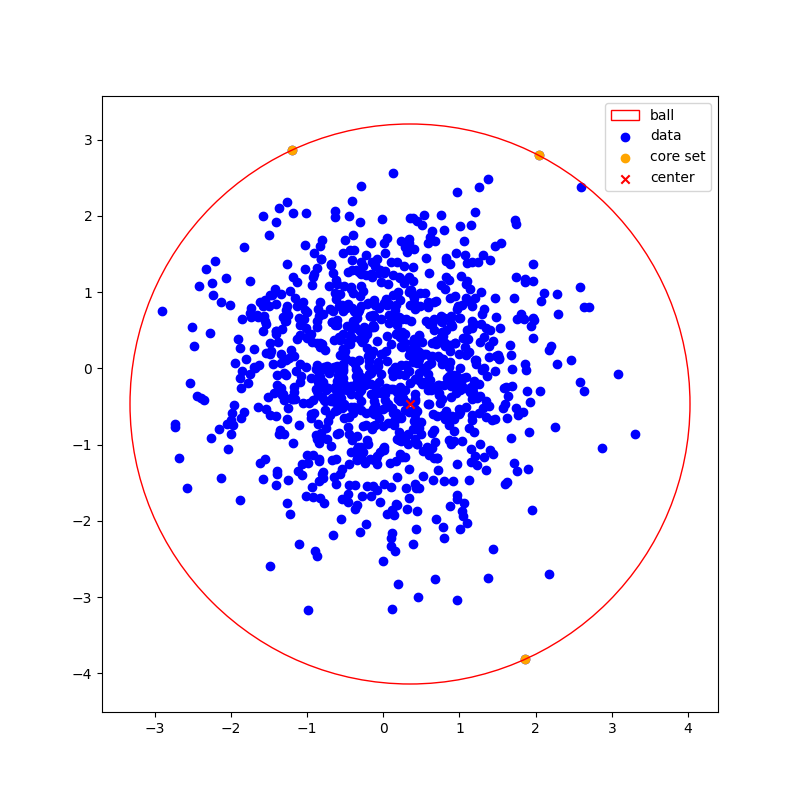
\includegraphics[width=0.5\textwidth]{core_set_example.png}
    \caption{Example of a Core-Set for an MEB}
    \label{fig:core set example}
\end{figure}

\section{Minimum Enclosing Ball with Outliers}
\subsection{Formulation}
\begin{definition}\label{mebwo}
    We may extend Definition \ref{meb} to the Minimum Enclosing Ball with Outliers (MEBwO) problem as follows:
    \begin{center}
        \begin{tabular}{CCC}
             \displaystyle\min_{c,r,\xi} & r \\
             \text{s.t.} & \norm{c-a^i} \leq r + M\xi_i, & i=1,\ldots,n, \\
             & \displaystyle\sum_{i=1}^n\xi_i \leq k, \\
             & \xi_i \in \binary, & i=1,\ldots,n.
        \end{tabular}
    \end{center}
    
    where $\xi_i$ are binary variables corresponding to the distance constraint on each variable, with $M\in\mathbb{R}$ a sufficiently large scalar. One can interpret this as, if $\xi_i=1$ for some $i\in\left\{1,\ldots,n\right\}$, then $a_i$ does not need to be inside the ball. The constraint $\sum_{i=1}^n\xi_i\leq k$ where $k=\floor{n(1-\eta)}$ ensures that $\eta\%$ of the data is covered.
    
    We can instead extend the QCQP in Definition \ref{meb} to get the following mixed integer QCQP (MIQCQP) formulation:
    \begin{center}
        \begin{tabular}{CLC}
            \displaystyle\min_{c,\gamma, \xi} & \gamma \\
            \text{s.t.} & \left(a^i\right)^Ta^i - 2\left(a^i\right)^Tc + c^Tc \leq \gamma + M\xi_i & i=1,\ldots,n \\
            & \displaystyle\sum_{i=1}^n\xi_i \leq k \\
            & \xi_i \in \binary & i=1,\ldots,n
        \end{tabular}
    \end{center}
\end{definition}
\begin{remark}
    One may note that when we relax $\xi_i$ to be continuous variables, i.e. $0\leq\xi_i\leq1$ for $i=1,\ldots,n$, we have again a convex QCQP since we have then added only continuous variables and linear constraints to the base QCQP.
\end{remark}

This model gives us a way to solve the MEBwO problem optimally for a given data set. However, by examining the structure of this model we can expect the solution times to be unreasonable for any meaningfully large instance. Note that, of $n$ many binary variables $\xi_i$, we can choose up to $k\leq n$ many of them to have a value of 1, though by Proposition \ref{removing data} we know that removing data gives us an MEB with potentially lower radius, meaning we will always pick the highest possible number of points ($k$ many) to be excluded. Thus, by a total brute force search we may expect to explore $\binom{n}{k}$ many individual MEB problems. Modern optimization solvers will work more efficiently than this, utilizing techniques such as branch-and-bound. Regardless, we expect a very large solution space which leads to exponentially larger solution times as we will see in Section \ref{exact benchmarks}.


\subsection{On the Big-M Parameter}\label{sec:M}
The ``big $M$ constraint" in Definition \ref{mebwo} is a commonly known technique within Operational Research and an important question is that of what $M$ do we choose? A sufficiently large $M$ is required such that when the corresponding binary variable is equal to $1$, the constraint is effectively nullified. But, as we will see within this section, a value of $M$ which is too large will lead to a longer solution time with worse solutions.

\subsubsection{An Upper Bound on $M$}
Finding a suitable value of $M$ depends heavily on the nature of the problem the constraint is being applied to. For the minimum enclosing ball with outliers problem, where we are concerned with the distances $\norm{c-a^i}$ being less than the radius $r$, we look to add a value to $r$ such that for any reasonable $c$, this constraint is always satisfied. Thus, a candidate upper bound for $M$ may be found by calculating each pairwise distance within the data and recording the largest distance. Formally, this may be written as $M:= \max\left\{\norm{a^i-a^j}: i,j = 1,\ldots,n, i\neq j\right\}$.

An immediately apparent issue with this approach is that computing $M$ in this way will run in $O(n^2d)$ time. For smaller data sets this is manageable, but for any significantly sized data sets the time taken to compute $M$ is often longer than the time taken to solve the MEBwO problem on the same data.

We can look to \cite[Lemma 1]{core-sets} for a $1/\sqrt{3}$-approximation to the diameter of $\A$ which runs in $O(nd)$ time, by picking a random point $p\in\A$, finding $q$ the furthest point in $\A$ from $p$, finding $q'$ the furthest point in $\A$ from $q$, then setting $D:=\norm{q-q'}$ which is our $1/\sqrt{3}$-approximation to the diameter of $\A$. For a candidate $M$ value we can simply set $M:=\sqrt{3}D$.

\begin{algorithm}[H]\label{alg:diameter approx}
    \KwIn{Data set $\A$, point $p\in\A$}
    \KwOut{Approximate diameter $D\in\mathbb{R}$}
    $q:=\arg\max_{a\in\A}\norm{p-a}$\;
    $q':=\arg\max_{a\in\A}\norm{q-a}$\;
    $D:=\norm{q-q'}$\;
    \KwRet{D}\;
    
    \caption{Diameter Approximation Algorithm \cite[Lemma 1]{core-sets}}
\end{algorithm}
A caveat to this approach is that it the value of $M$ will change depending on the initial random point chosen, and can vary significantly. To demonstrate this, we generate a standard normal data set $\A$ with $n=1000$, $d=10$ (see Section \ref{data}), and by running Algorithm \ref{alg:diameter approx} for each $a\in\A$ we construct a distribution of approximate diameters. From \texttt{src/diameter\_approx\_analysis.py} we find an average diameter of $8.939$ with variance $0.170$ and a density plot is shown in Figure \ref{fig:diameter approx density}.
TODO: report actual diameters and change M on x axis to diameter
\begin{figure}
    \centering
    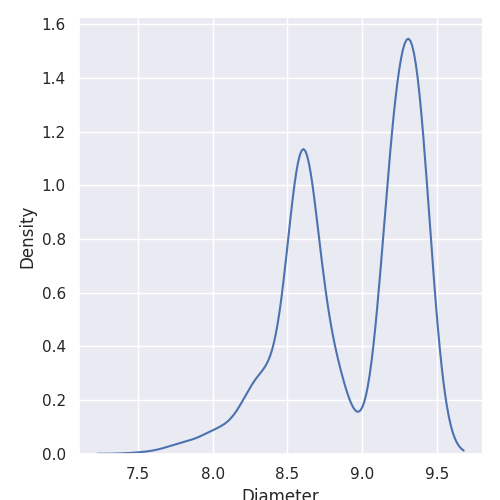
\includegraphics[width=0.5\textwidth]{pw_M_density.png}
    \caption{Density Plot of Approximate Diameters from Algorithm \ref{alg:diameter approx}}
    \label{fig:diameter approx density}
\end{figure}

For more robust benchmarking, we would prefer a method which always returns the same $M$ value for a given data set, so this method is unsuitable for our purposes. This is because, as seen in the previous section, a higher value of $M$ has a negative effect on the run time of the solver so we would prefer to minimize the effect of randomness on our benchmarks.

Our chosen method, which gives reliable estimates for $M$ in a reasonable time is to simply solve the MEB problem for $\A$ and set $M:=2r$ for $B(c,r)=\MEB(\A)$. We know from Theorem \ref{thm:unique} that an MEB always exists and is unique for a given data set, so can always expect to receive the same $M$ value from this method. Using a heuristic approach such as Algorithm \ref{core-set algorithm} gives us a $(1+\epsilon)$-approximation to $\MEB(\A)$, so we will receive an $M$ value that is slightly larger than needed, but the effect on run time is insignificant and given that the returned $M$ value is consistent we do not introduce unneeded randomness into our methodology that is not already inherently present due to using randomly generated data.

\subsubsection{Solution Times}
One concern with our choice of $M$ is the effect on the solution time of the solver. Typically a larger than necessary value of $M$ will result in longer solution times, and so this is a concern given that our heuristics are intended to return a feasible solution to the MEBwO problem in reasonably fast time. In our benchmarking of solving the exact model we observe a significant increase in solution time as the value of $M$ increases when solving the exact model on the same data set (Figure \ref{fig:exact_benchmarks_M}). 

\subsubsection{Quality of $\xi_i$ Solutions in the QP Relaxation}
Another concern regarding the value of $M$ for the exat model is the effect on the optimal solutions for the relaxed $\xi_i$ variables in the QP relaxation. This is important as good quality relaxed solutions are essential to Algorithm \ref{relaxation heuristic}, which uses high-valued $\xi_i$ as a proxy for how far a data point lies from the optimal center, and so for how much of an outlier that point is.

We can evaluate the quality and diversity of relaxed solutions by solving the relaxed model on the same data set with different values of $M$. We generate random data sets (see Section \ref{data}) with $n=1000$, $d=10$, and the standard parameters described in Section \ref{data}, then calculate a lower bound for $M^*$ using Algorithm \ref{alg:diameter approx} for each data set, then solve the model for a sequence of multiples of $M^*$ and record the variance of the list of relaxed solutions. We choose to test 50 different values of $M$ in the sequence $\langle M^*(1+k/2)\rangle _{k=1,\ldots,50}$. The implementation can be found in \texttt{src/xi\_analysis.py} and a plot of the variances can be seen in Figure \ref{fig:xi analysis}.

\begin{figure}
    \centering
    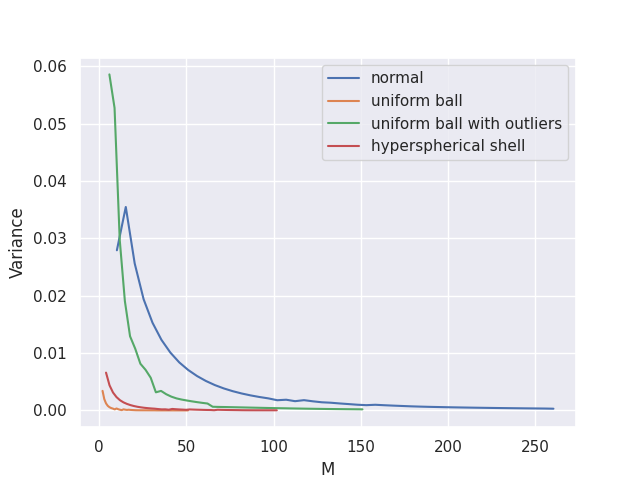
\includegraphics[width=0.75\textwidth]{xi_analysis.png}
    \caption{Variance of Relaxed $\xi_i$ Variables for a Sequence of $M$ Values.}
    \label{fig:xi analysis}
\end{figure}

We can see in Figure \ref{fig:xi analysis} that, for each data set, the variance of the relaxed solutions for $xi_i$ decreases sharply as $M$ increases and tends to zero. Interestingly there is actually a slight increase in variance at first for the normal data, but like the rest this does still tend to zero.

\section{Literature Review}\label{lit review}
We will now conduct a review of the current literature on the MEBwO problem.

Early approaches were developed specifically for the $d=2$ case of finding the minimum enclosing circle with outliers. One such paper is \cite{AGGARWAL199138} which discusses computing Voronoi cells and then performing a search of the resulting Voronoi cells. \cite{efrat} makes use of a parametric search technique proposed by \cite{megiddo}, and \cite{MATOUSEK1995217} uses a randomized search algorithm. These papers all gave exact solutions to the MEBwO problem in the two-dimensional case, while \cite{harpeled} presents some approximate algorithms.

Some more recent approaches are as follows. \cite{SHENMAIER201581} proves the NP-hardness of the MEBwO problem in Euclidean space (Theorem 1) and also that no fully polynomial time approximation scheme exists for the MEBwO problem unless $P=NP$ (Theorem 3). Shenmaier's paper also proposes two algorithms for solving the MEBwO problem in $\mathbb{R}^d$ which both have an approximation guarantee. We implement and benchmark Algorithm 1 in this paper which Shenmaier proves to give 2-approximate solutions, meaning we may get a lower bound on the optimal value of the MEBwO problem for a given data set. This algorithm works by computing the $k$-nearest points to each point in the data set and returning the smallest ball found. The second algorithm, not implemented in this paper, is an extension of the prior algorithm where a grid of candidate centres is constructed in a local neighbourhood of each point. This algorithm provides a tighter approximation guarantee but has significantly worse time complexity. Shenmaier also discusses the dual of the MEBwO problem, and the hardness of this dual is an interesting area of further research.

\cite{cavaleiro} presents an algorithm built on branch-and-bound \cite{bnb} which orders the nodes of the tree in such a way that along with a first-in-first-out search strategy results in a small number of nodes explored. \cite{huding} also presents a branch-and-bound algorithm, this time using the idea of core-sets and a bi-criteria approximation with respect to both the radius and percentage of points covered. This paper also utilizes the algorithm as a classification model on the MNIST \cite{lecun2010mnist} data set (for further details please see Section \ref{data}).

Due to the time constraints of this project and the difficulty of implementing branch-and-bound methods we will not be implementing these branch-and-bound algorithms in this paper, and instead focus on methods which work from a more geometric mindset. We will implement Shenmaier's approximation and also investigate some improvement heuristics which may be run quickly in order to improve the initial solution provided from this method.








% =============================================================================
% Chapter 3
% =============================================================================

\chapter{Heuristic and Approximation Algorithms}\label{algorithms}

In this chapter we propose some non-exact construction methods to solving the MEBwO problem which return a feasible solution. We also investigate some improvement heuristics which, given a feasible MEB or MEBwO, seek to locally find a new center such that a smaller radius can be found.

\section{Construction Methods}
\subsection{Relaxation-Based Heuristic}
This heuristic works by first solving the relaxed QP formulation for the MEBwO problem in Definition \ref{mebwo}, and then making the assumption that a higher value of $\xi_i$ (i.e. closer to 1) means that the model treats the data point $a^i$ as ``more" of an outlier. From this assumption, we pick the largest $k$ values of $xi_i$ and treat each corresponding $a^i$ as an outlier, therefore treating the remaining data as inliers. We then solve the MEB problem for this remaining data. A more formal outline of this algorithm is detailed in Algorithm \ref{relaxation heuristic}.

This method will always return a feasible solution that covers $\eta\%$ of the data as we will always remove $k=\floor{n(1-\eta)}$ many points. As discussed in the previous chapter, solving the final MEB problem is relatively easy and selecting outliers using the MEBwO QP relaxation is trivial, but the difficulty lays in solving the initial QP relaxation, and as such a heuristic method which can solve this model quickly and return approximate solutions to each $xi_i$ is a valuable direction for further research in order to speed up this method.

\begin{algorithm}[H]\label{relaxation heuristic}
    \SetAlgoLined
    \KwIn{Data set $\A=\left\{a^1,\ldots,a^n\right\}$, percentage of data to be covered $\eta\in[0,1]$, error tolerance for MEB heuristic $\epsilon>0$, big $M$ parameter $M>0$}
    \KwOut{Ball $B(c,r)$}
     $\xi=\left[\xi_1,\ldots,\xi_n\right]$ the relaxed binary variables returned by relaxed MEBwO solver for $\A$, $\eta$, and $M$\;
     Let $\xi'$ be the smallest $k=\floor{\eta\cdot n}$ elements of $\xi$\;
     Let $\A':=\left\{a^i\in\A: \xi_i\in\xi',\ i=1,\ldots,n\right\}$\;
     Let $c,r$ be the center and radius of $\MEB(\A')$ returned by heuristic\;
     \KwRet $B(c, r)$\;
     
    \caption{Relaxation-Based Heuristic}
\end{algorithm}

\subsection{Shenmaier's Approximation}
\subsubsection{Statement}
This approximation scheme developed by Vladimir Shenmaier in \cite[Algorithm 1]{SHENMAIER201581} is a brute-force algorithm to solving the MEBwO problem with $O(n^2d)$ time complexity. It works by considering each point in the input set, finding the $k$-closest points to that point, then returning the point-distance pair such that the maximum distance from each point to each other point in its $k$-closest points is minimised. See Algorithm \ref{shenmaier} for a detailed outline of this algorithm.
\begin{algorithm}
    \KwIn{Data set $\A$, $\eta\in[0,1]$}
    \KwOut{Ball $B(c,r)$}
    $k=\floor{n(1-\eta)}$\;
    \For{$i=1,\ldots,n$}{
        $D:=\left\{\norm{a^i-a}: a\in\A\right\}$\; % TODO: FIX THIS
        Let $D'$ be $D$ sorted in ascending order\;
        Let $\delta_i$ be the $(k-1)$th element of $D'$ (indexing from 0)\;
    }
    $i^* := \arg\min_{i=1,\ldots,n}\delta_i$\;
    $c := a^{i^*}$\;
    $r := \delta_{i^*}$\;
    \KwRet{$B(c,r)$}\;
    
    \caption{Shenmaier's Approximation \cite[Algorithm 1]{SHENMAIER201581}}
    \label{shenmaier}
\end{algorithm}
\subsubsection{Approximation Guarantee} %TODO: could make this a theorem
 From \cite[Theorem 4]{SHENMAIER201581} we know that Algorithm \ref{shenmaier} returns a 2-approximation solution to the MEBwO problem. What this means is that if we have a minimum radius of $r$ returned by Algorithm \ref{shenmaier} for a data set $\A$, then the true optimal value to the MEBwO problem on that data is no less than $r/2$. This is useful for assessing how close a heuristic is to an optimal solution in the worst case when we have a solution via Algorithm \ref{shenmaier}, but not an optimal solution via solving the exact model.

\subsubsection{Complexity}
Referring to Algorithm \ref{shenmaier}, on line 1 we have an assignment which runs in $O(1)$ time. On lines 2 through 5 we have a \texttt{for} loop which runs $n$ many times, and on line 3 we compute a list of $n$ many distances, which for $d$-dimensional vectors runs in $O(nd)$ time. Line 4 involves sorting the aforementioned list, so the time complexity depends on the sorting algorithm used. It is well known within computer science that algorithms are often subject to a time-memory trade off, meaning that it is possible to design algorithms that run faster as a result of using less memory, and vice-versa. We can then assume that a sensible implementation of Algorithm \ref{shenmaier} would use the fastest available sorting algorithm given that the size of our data sets are small enough that we do not run into memory constraints, so the recommended sorting algorithm is Quicksort \cite{hoare1962quicksort} which runs on average in $O(n\log n)$ time. Line 5 simply accesses the $(k-1)$th element of the sorted list and so runs in $O(1)$ time.

Line 6 finds the minimum element from a set of values and runs in $O(n)$ time. Lines 7 and 8 are simple assignments and run in $O(1)$ time. Finally, our overall time complexity is then $O(n^2(d+\log n))$. This will usually reduce to $O(n^2d)$ as typically $d>\log n$, though for particularly large $n$ and very small $d$ the alternative reduction of $O(n^2\log n)$ is of course possible.

\subsection{MEB Shrinking Heuristic}
\subsubsection{Statement}
The MEB Shrinking Heuristic works by computing $\MEB(\A) = B(c,r)$, then simply shrinking the radius until $\eta\%$ of points are covered. This is done by calculating the $n-k$ closest points to $c$ and returning the ball $B(c,r')$ where $r'$ is the greatest distance from $c$ to each of the $n-k$ points.

\begin{algorithm}[H]\label{meb shrink}
    \SetAlgoLined
    \KwIn{Data set $\A$, $\eta\in[0,1]$, $\epsilon>0$}
    \KwOut{Ball $B(c,r)$}
    $k:=\floor{n(1-\eta)}$\;
    Let $c$ be the center of the MEB returned by a heuristic for $\MEB(\A)$\;
    $D:=\left\{\norm{c-x}: x\in\A\right\}$\;
    Let $D'$ be $D$ sorted in ascending order\;
    Let $\delta$ be the $(k-1)$th element of $D'$ (indexing from 0)\;
    $\A' = \left\{a^i\in\A: D[i] \leq \delta, i=1,\ldots,n\right\}$\;
    $r = \max_{a\in\A'}\norm{c-a}$\;
    \KwRet $B(c,r)$\;
    
    \caption{MEB Shrinking Heuristic}
\end{algorithm}

\subsubsection{Complexity}
The complexity of this heuristic mostly depends on the choice of heuristic for solving the MEB problem on $\A$. The dominant term in lines 3 though 7 is on average $O(n\log n)$ from sorting the list of distances, so the overall complexity is the greater out of this and the complexity of the heuristic. Our implementation uses Algorithm \ref{core-set algorithm}, which in this case is $O\left(\frac{nd}{\epsilon}+\frac{d^2}{\epsilon^{3/2}}\left(\frac{1}{\epsilon}+d\right)\log\frac{1}{\epsilon}\right)$ \cite[Page 6]{core-sets}.
\subsection{Average Point Heuristic}
\subsubsection{Statement}
The Average Point Heuristic (APH) works by finding the average point, i.e. $c=\frac{1}{n}\sum_{i=1}^n a^i$, then finding the $n-k$ closest points and returning the ball $B(c,r)$ where $r$ is the greatest distance from $c$ to each of the $n-k$ points.

\begin{algorithm}[H]\label{avg point shrink}
    \SetAlgoLined
    \KwIn{Data set $\A$, $\eta\in[0,1]$}
    \KwOut{Ball $B(c,r)$}
    $k:=\floor{n(1-\eta)}$\;
    $c:=\frac{1}{n}\sum_{i=1}^na^i$\;
    $D:=\left\{\norm{c-x}: x\in\A\right\}$\;
    Let $D'$ be $D$ sorted in ascending order\;
    Let $\delta$ be the $(k-1)$th element of $D'$ (indexing from 0)\;
    $r = \max_{a\in\A'}\norm{c-a}$\;
    \KwRet{$B(c,r)$}
    
    \caption{Average Point Shrinking Heuristic}
\end{algorithm}

\subsubsection{Complexity}
This algorithm runs extremely quickly, with the dominating term in the time complexity being $O(nd\log n)$ on average as a result of sorting the list of distances on line 4, so when . TODO: what is this This is far faster than any other construction method and is more resistant to outliers than the MEB shrinking heuristic.
%TODO: can order the algorithms in order of complexity
%TODO: talk about how improvement heuristics can be used after each heuristic except the relaxation-based heuristic since it finds and MEB so minimum

\section{Improvement Heuristics}\label{sec:improvement_heuristics}
We now consider some improvement heuristics. The two heuristics described here are, strictly speaking, designed to improve an existing MEB rather than an MEBwO. However, quick and effective methods exist for solving the MEB problem and so improvement heuristics have not been needed, while heuristics which solve the MEBwO problem may return a solution which has considerable space for improvement. %TODO: not talking about MEB

The two improvement heuristics work in a similar way, by considering an improving direction in which moving the centre of the MEB in that direction while keeping the same radius retains a feasible solution, then shrinking the radius to the furthest point from the new centre. The Direction-Constrained Single Step Heuristic (DCSSH) works by pure geometric reasoning to find a new centre, while the Direction-Constrained MEB (DCMEB) uses an optimization solver such as Gurobi to find an optimal step in the improving direction to minimize the radius of the new ball.

The inspiration for these heuristics comes from Shenmaier's Approximation, which returns a ball with some centre $c\in\A$. Our assumption is that a better solution exists in a local neighbourhood around $c$, i.e. we find a new centre that does not have to lie on a point in $\A$. Both heuristics consider only a single step, but as they are quick to run we may run each heuristic in succession to build a sequence of steps that lead to an improved solution. There are various stopping criteria one could consider in an implementation of these heuristics, such as setting an iteration limit or stopping once each iteration yields an improvement below some threshold. For ease of implementation we will choose the iteration limit since each iteration is computationally cheap.

For an example of this refer to Figure \ref{fig:riterations} which shows the new radius after each iteration of each improvement heuristic on each data set for $n=1000$, $d=100$, and the standard parameters for each data type (see Section \ref{data}). These examples were run on one data set each rather than averaged over multiple data sets and so should not be used to draw any conclusions.

\subsection{Direction-Constrained Single Step Heuristic}
\subsubsection{Derivation}
For a visual aid to this derivation please refer to Figure \ref{vis aid derivation}. Consider $B(\hat{c}, r) = \MEB(\A)$. To find an improving direction we choose the furthest point from $c$, $\hat{a}=\arg\max_{a\in\A}\norm{c-a}$, then the (negative) improving direction is defined to be $\beta=\hat{c}-\hat{a}$. We choose the direction $\hat{a}\to\hat{c}$ as opposed to $\hat{c}\to\hat{a}$ in order to simplify later derivations.

Now that we have a direction $\beta$, we can move the initial ball in this direction by simply subtracting $\beta x$ from $\hat{c}$ where $x\in\mathbb{R}^{\geq0}$ is some scalar, i.e. our new centre is $c=\hat{c}-\beta x$. We would like to choose $x$ such that the new ball remains feasible by ensuring that $\norm{c-a^i}\leq r$ for $i=1,\ldots,n$, and we can do this by considering the distance from each $a^i$ in the direction of $\beta$ to the surface of the initial ball and choose $x$ such that each of these distances is greater than $\norm{\beta x}$.

More formally, for each $a^i\in\A$ let $x_i$ be the scalar such that $a^i+\beta x_i$ lies on the surface of the initial ball, i.e. $\norm{(a^i+\beta x^i)-\hat{c}}=r$. Again, to simplify derivations, denote the direction $\hat{c}\to a^i$ by $\alpha_i=a^i-\hat{c}$. To calculate each $x_i$, we square this equation and set $\gamma=r^2$ to get
\begin{align*}
    \alpha_i^T\alpha_i + 2x\alpha_i^T\beta + x^2\beta^T\beta &= \gamma \\
    \implies \beta^T\beta x^2 + 2\alpha_i^T\beta x + \alpha_i^T\alpha_i - \gamma &= 0.
\end{align*}
Using the quadratic formula we then have
\begin{align*}
    x &= \frac{-2\alpha_i^T\beta \pm \sqrt{4\left(\alpha_i^T\beta\right)^2 - 4\beta^T \beta\left(\alpha_i^T\alpha_i-\gamma\right)}}{2\beta^T\beta} \\[4pt]
    &= \frac{-\alpha_i^T\beta \pm \sqrt{\left(\alpha_i^T\beta\right)^2 - \beta^T \beta\left(\alpha_i^T\alpha_i-\gamma\right)}}{\beta^T\beta}.
\end{align*}
The two solutions to $x$ corresponding to the positive and negative discriminants represent the steps in the positive and negative $\beta$ directions respectively, then since from our derivations we are only interested in the positive $\beta$ direction we can disregard the negative solution for $x$, so we can define the function $Q:\mathbb{R}^d\times\mathbb{R}^d\times\mathbb{R}\to\mathbb{R}$ by
\begin{equation*}
    Q(\alpha_i,\beta,\gamma) = \frac{-\alpha_i^T\beta + \sqrt{\left(\alpha_i^T\beta\right)^2 - \beta^T \beta\left(\alpha_i^T\alpha_i-\gamma\right)}}{\beta^T\beta}.
\end{equation*}


Then let $x=\min\left\{Q(\alpha_i, \beta, \gamma):i=1,\ldots,n\right\}$, so $\norm{\beta x}$ is the smallest distance from each $a^i$ to the surface of the ball in the direction of $\beta$. Finally, by moving by some scalar multiple of $-\beta x$ from $\hat{c}$, we get a new feasible centre $c=\hat{c}-\beta x/s$ for some scalar $s\geq1$. We give a simple proof that this new centre with unchanged radius indeed yields a feasible solution and a visual aid is provided in Figure \ref{vis aid feasibility}. See Algorithm \ref{fig:dcssh} for a detailed outline of this algorithm.

\begin{figure}
    \centering
    \begin{tikzpicture}
        % lines
        \draw[->, color=magenta] (-3,0) -- (-0.05,0) node[midway, below]{$\beta$};
        \draw[->, color=cyan] (0,0) -- (59/60,59/40) node[midway, below right]{$\alpha_i$};
        \draw[dashed] (1,1.5) -- (2.598, 1.5) node[midway, below]{$\norm{\beta}{x}$};
        
        % points
        \draw[fill] (0,0) circle (1.5pt) node[below]{$\hat{c}$};
        \draw[fill] (-3,0) circle (1.5pt) node[left]{$\hat{a}$};
        \draw[fill] (1, 1.5) circle (1.5pt) node[above left]{$a^i$};
        \draw[fill] (2.598, 1.5) circle (1.5pt) node[above right]{$a^i + \beta x$};
        \draw[fill] (-0.75,0) circle (1.5pt) node[above]{$\hat{c}-\frac{\beta x}{s}$};

        % ball
        \draw (0,0) circle (3);
    \end{tikzpicture}
    \caption{Visual Aid for Direction-Constrained Single Step Heuristic}
    \label{vis aid derivation}
\end{figure}

\begin{proposition}\label{imp heuristic feasibility}
Consider the MEB problem for a data set $\A$ denoted by $(P)$. Let $B(\hat{c},r)$ be a feasible solution to $(P)$. Then the ball $B(\hat{c}-\beta x/s, r)$ with $\beta$, $x$, and $s$ as described above, is also a feasible solution to $(P)$.
\end{proposition}
\begin{proof}
For each $a^i\in\A$ let $\hat{a}^i_\beta$ be the point on the surface of $B(\hat{c},r)$ in the direction of $\beta$ from $a^i$. Let $a^i_\beta=\hat{a^i}_\beta - \beta x/s$ be the point on the surface of $B(\hat{c}-\beta x/s, r)$ in the direction of $\beta$ from $a^i$. Let $c=\hat{c}-\beta x/s$. Then, by the triangle inequality, we have
\begin{align*}
    \norm{c-a^i_\beta} &\geq \norm{c-a^i} + \norm{a^i-a^i_\beta} \\
    \implies \norm{c-a^i} &\leq \norm{c-a^i_\beta} - \norm{a^i-a^i_\beta} \\
    &= r-\norm{a^i-a^i_\beta} \\
    &\leq r
\end{align*}
since $\norm{a^i-a^i_\beta}\geq0$. Hence $\norm{c-a^i}\leq r$ for $i=1,\ldots,n$ and so $B(c, r)$ is feasible for $(P$).
\end{proof}

\begin{algorithm}[H]\label{fig:dcssh}
    \KwIn{Data set $\A$, Ball $B(\hat{c},\hat{r})$, scalar $s\geq1$}
    \KwOut{Ball $B(c,r)$}
    $\hat{a}:=\arg\max_{a\in\A}\norm{\hat{c}-a}$\;
    $\beta:=\hat{c}-\hat{a}$\;
    $\gamma:=\hat{r}^2$\;
    \For{$i=1,\ldots,n$}{
        $\alpha_i:=a^i-\hat{c}$\;
        $x_i:=Q(\alpha_i, \beta, \gamma)$\;
    }
    $x:=\min\left\{x_i: i=1,\ldots,n\right\}$\;
    $c:= \hat{c}-\beta x/s$\;
    $r:=\max_{i=1,\ldots,n}\norm{c-a^i}$\;
    \KwRet{$B(c,r)$}\;
    \caption{Direction-Constrained Single Step Heuristic}
\end{algorithm}
\begin{figure}
    \centering
    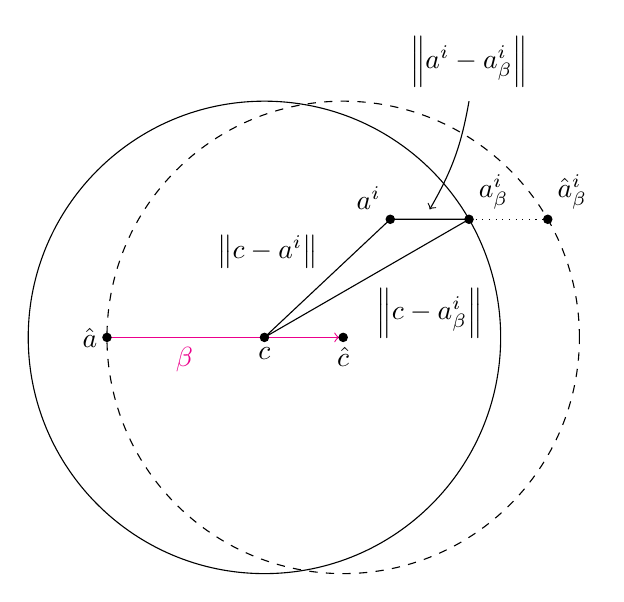
\begin{tikzpicture}
        % lines
        \draw (0,0) -- (1.598, 1.5) node[midway, above left]{$\norm{c-a^i}$} -- (2.598, 1.5) -- cycle node[midway, below right]{$\norm{c-a^i_\beta}$};
        \draw[dotted] (2.598, 1.5) -- (3.598, 1.5);
        
        \draw[->, color=magenta] (-2,0) -- (0.95,0) node[pos=0.3333, below]{$\beta$};
        
        % points
        \draw[fill] (0,0) circle (1.5pt) node[below] {$c$};
        \draw[fill] (-2,0) circle (1.5pt) node[left]{$\hat{a}$};
        \draw[fill] (1,0) circle (1.5pt) node[below]{$\hat{c}$};
        
        \draw[fill] (1.598, 1.5) circle (1.5pt) node[above left]{$a^i$};
        \draw[fill] (2.598, 1.5) circle (1.5pt) node[above right]{$a^i_\beta$};
        \draw[fill] (3.598, 1.5) circle (1.5pt) node[above right]{$\hat{a}^i_\beta$};
        
        % balls
        \draw (0,0) circle (3);
        \draw[dashed] (1,0) circle (3);
        
        % labels
        \node at (2.598, 3.5) {$\norm{a^i-a^i_\beta}$};
        \draw[->] (2.598, 3) to[bend left=10] (2.098, 1.625);
        % TODO: make it clear that a^ibeta are not points
    \end{tikzpicture}
    \caption{Visual Aid for Proposition \ref{imp heuristic feasibility}}
    \label{vis aid feasibility}
\end{figure}
\subsubsection{Complexity}

The complexity of the DCSSH is easy to determine. Referring to Algorithm \ref{fig:dcssh}, on line 1 we have a loop over each data point which runs in $O(n)$ time. On lines 4 through 6 we have a \texttt{for} loop which runs $n$ many times, with the operations on lines 5 and 6 both being $O(d)$ as they are each single operations on $d$-dimensional vectors, so overall this loop runs in $O(nd)$ time. On lines 7 and 8 we find the minimum and maximum of two lists respectively, again $O(n)$. Finally, on line 8, a single operation on $d$-dimensional vectors runs in $O(d)$ time. Our dominating term is then $O(nd)$.
\subsection{Direction-Constrained MEB Heuristic}
\subsubsection{Derivation}
For a visual aid to this derivation please refer to Figure \ref{fig:dcmeb}. Consider $B(\hat{c},\hat{r})$. Similarly to the DCSSH, for an improving direction we choose the furthest point in $\A$ from $\hat{c}$, $\hat{a}=\arg\max_{a\in\A}\norm{\hat{c}-a}$, and let $\beta=\hat{a}-\hat{c}$ be this direction. Note that this is the negative of $\beta$ used in the derivation of the DCSSH, as we are now considering the direction $\hat{c}\to\hat{a}$. Now, instead of calculating distances between each point in data and the surface of the ball to find a feasible step length from $\hat{c}$ towards $\hat{a}$, we formulate an optimization model to find an optimal step length such that the new ball still contains all data, but has a smaller radius.

We modify the optimization model for the MEB problem, adding the constraint that $c$ must lie on the direction $\beta$ from $\hat{c}$. It is possible to formulate this exactly using the constraint $c=x(\hat{c}+\beta)$, however a better formulation is to consider a variable $x\in\mathbb{R}^{\geq0}$, then write $c=\hat{c}+\beta x$. Obviously $\hat{c}$ is a constant vector so this reduces the problem of finding the new $c$ to that of finding the optimal solution to one variable $x$, as opposed to $d$ many decision variables for each element of the vector $c$. The optimization model for the DCMEB problem is as follows:
\begin{center}
    \begin{tabular}{CCC}
        \displaystyle\min_{x,r} & r \\
        \text{s.t.} & \norm{\hat{c}+\beta x - a^i} \leq r & i=1,\ldots,n \\
        & x\geq0
    \end{tabular}
\end{center}

By setting $\gamma=r^2$, $\alpha^i=\hat{c}-a^i$ for $i=1,\ldots,n$, and squaring the norm constraints, we get the following QCQP:
\begin{center}
    \begin{tabular}{CCC}
        \displaystyle\min_{x,\gamma} & \gamma \\
        \text{s.t.} & \beta^T\beta x^2 + 2\alpha_i^T\beta x + \alpha_i^T\alpha_i \leq \gamma & i=1,\ldots,n \\
        & x\geq0
    \end{tabular}
\end{center}

This model has $n+1$ constraints and most crucially, 2 decision variables. This makes the model extremely computationally easy to solve by modern solvers such as Gurobi. In fact, like the original MEB problem, we may formulate the DCMEB problem as as a SOCP by considering the cones
\begin{equation*}
    C_i = \left\{(r,\beta x+\hat{c}-a^i) \in \mathbb{R}^{d+1}: \norm{\beta x +\hat{c}-a^i}\leq\gamma\right\}.
\end{equation*}
and as such the DCMEB problem may be solved by interior-point methods \cite{socp_ipm}. The DCMEB heuristic is then to simply solve the DCMEB, given a data set $\A$ and initial ball $B(\hat{c},\hat{r}$, using the solutions of the solved DCMEB problem for the new ball.

\begin{algorithm}[H]
    \KwIn{Data set $\A$, Ball $B(\hat{c},\hat{r}$)}
    \KwOut{Ball $B(c,r)$}
    $\hat{a}:=\arg\max_{a\in\A}\norm{\hat{c}-a}$\;
    Let $x$, $r$ be the solutions returned by solver for the DCMEB problem for $B(\hat{c},\hat{r})$\;
    $c:=c+x(\hat{a}-\hat{c})$\;
    \KwRet{$B(c,r)$}\;
    \caption{Direction-Constrained MEB Heuristic}
\end{algorithm}

\begin{figure}
    \centering
    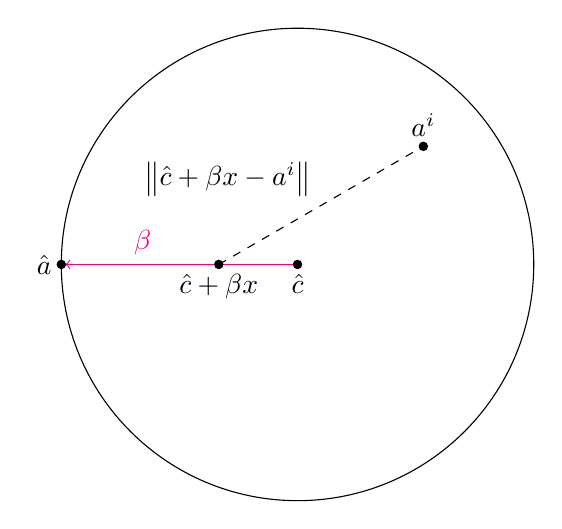
\begin{tikzpicture}
        % lines
        \draw[->, color=magenta] (0,0) -- (-2.95,0) node[pos=0.6666, above]{$\beta$};
        \draw[dashed] (-1,0) -- (1.598, 1.5) node[midway, above left]{$\norm{\hat{c}+\beta x - a^i}$};
        % points
        \draw[fill] (0,0) circle (1.5pt) node[below]{$\hat{c}$};
        \draw[fill] (-3,0) circle (1.5pt) node[left]{$\hat{a}$};
        \draw[fill] (1.598, 1.5) circle (1.5pt) node[above]{$a^i$};
        \draw[fill] (-1,0) circle(1.5pt) node[below]{$\hat{c}+\beta x$};
        
        % ball
        \draw (0,0) circle (3);
    \end{tikzpicture}
    \caption{Visual Aid for Derivation of the Direction-Constrained MEB}
    \label{fig:dcmeb}
\end{figure}

\subsubsection{Complexity}

The operations in this heuristic are simply finding a maximally distant point which runs in $O(nd)$ time, solving the DCMEB problem, and an assignment which runs in $O(1)$ time. So, the interest is in the time complexity of the method used to solve the DCMEB problem. As this problem is a SOCP it makes sense to apply interior-point methods which may then solve it in polynomial time (TODO: NEEDS CITATION).


\begin{figure}
    \centering
    \begin{subfigure}[b]{0.475\textwidth}
        \centering
        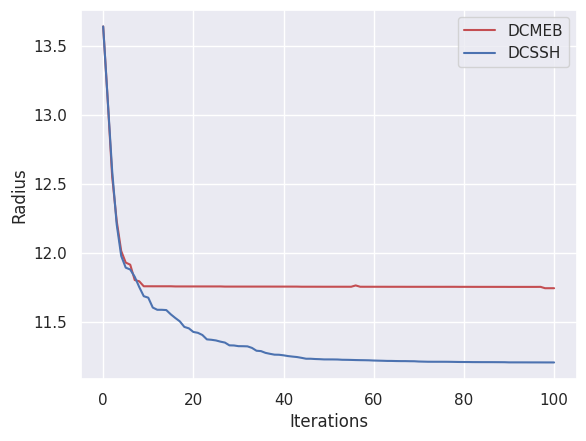
\includegraphics[width=\textwidth]{improvement_example/improvement_example_normal.png}
        \caption{Normal}
    \end{subfigure}
    \hfill
    \begin{subfigure}[b]{0.475\textwidth}
        \centering
        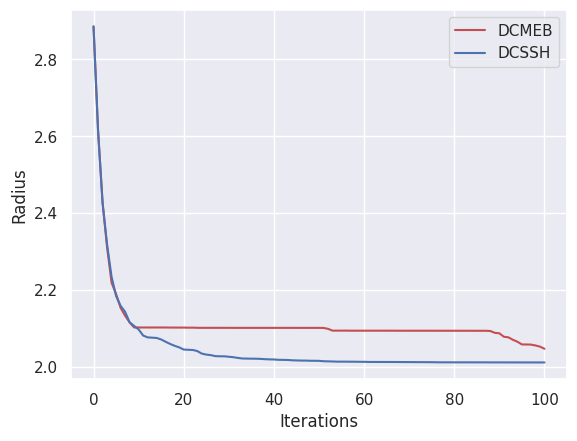
\includegraphics[width=\textwidth]{improvement_example/improvement_example_hyperspherical_shell.png}
        \caption{Hyperspherical Shell}
    \end{subfigure}
    \vskip\baselineskip
    \begin{subfigure}[b]{0.475\textwidth}
        \centering
        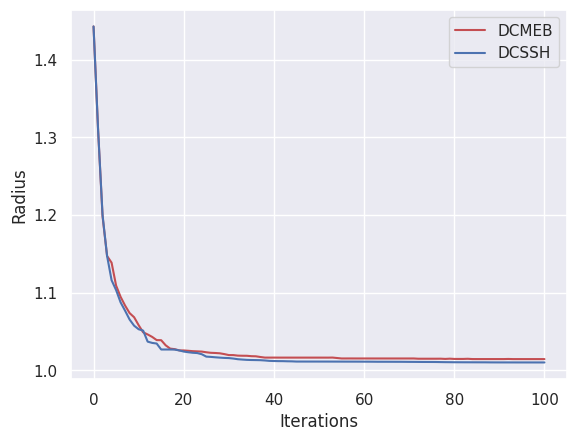
\includegraphics[width=\textwidth]{improvement_example/improvement_example_uniform_ball.png}
        \caption{Uniform Ball}
    \end{subfigure}
    \hfill
    \begin{subfigure}[b]{0.475\textwidth}
        \centering
        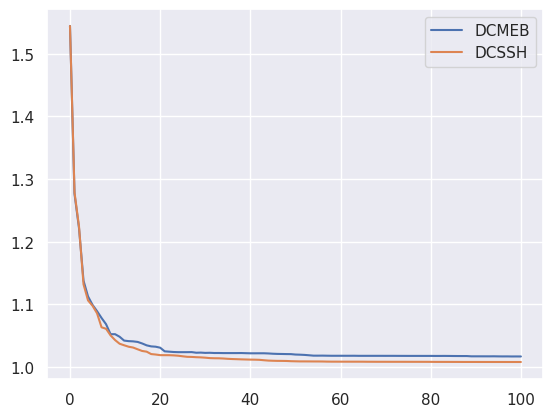
\includegraphics[width=\textwidth]{improvement_example/improvement_example_uniform_ball_with_outliers.png}
        \caption{Uniform Ball with Outliers}
    \end{subfigure}
    \caption{Reduction of Radius by each Iteration of Improvement Heuristics}
    \label{fig:riterations}
\end{figure}
% =============================================================================
% Chapter 4
% =============================================================================
\chapter{Implementation and Data}\label{implementation}
\section{Code}
\subsection{Software}\label{sec:software}
We implement our algorithms and data generation using Python 3.8 \cite{python}. Python is a high-level procedural programming language which is commonly used in data science and mathematics for its low barrier to entry, wide-scale adoption, and rich package ecosystem. One drawback of using Python is that it is known to be slow compared to other languages.

An implementation of our work in a faster programming language such as C \cite{kernighan2006c} will almost certainly result in faster run times --- in fact many Python packages such as scikit-learn \cite{scikit-learn} and NumPy \cite{numpy} utilize C to run the more time-consuming processes, and the Gurobi \cite{gurobi} solver is written in C while Python and other languages with Gurobi support are merely interfaces to this solver. A new up-and-coming programming language is Julia \cite{bezanson2017julia} which promises similar run times to C and has a mature library for interfacing with optimization solvers known as JuMP \cite{jump}. Due to the time constraints on this paper, we make use of the author's prior knowledge in Python for the implementation as previously mentioned but again acknowledge that there are indeed potentially superior choices for this type of work.

Packages within Python we make use of in the implementation are NumPy \cite{numpy} for numerical computation and linear algebra, pandas \cite{pandasjeff_reback_2021_5060318}{pandasmckinney-proc-scipy-2010} for data manipulation, Matplotlib \cite{matplotlib} and Seaborn \cite{seaborn} for visualisation and plotting, and finally TensorFlow Datasets \cite{TFDS} to access the MNIST \cite{lecun2010mnist} data set.

For modelling and solving our exact models for the MEBwO and DCMEB problems we use the Gurobi optimization solver \cite{gurobi}. At the time of writing, Gurobi is one of the fastest and most powerful mathematical programming solvers available and in particular is able to formulate and solve the QCQP and MIQCQP problems we require, so Gurobi was an easy choice of solver. Gurobi also has an easy to use Python interface which we make use of in our implementation.

\subsection{Implementation}
Our implementation can be found on Github \footnote{\url{https://github.com/tomholmes19/Minimum-Enclosing-Balls-with-Outliers} \cite{Holmes_Minimum_Enclosing_Balls_2021}} within the \texttt{src} folder and overall consists of around 2000 lines of code. All scripts used to run benchmarks and create figures are contained within this folder, and we have also written three packages contained therein. The \texttt{meb} package contains an object-oriented framework for MEB objects, defining \texttt{Ball}, \texttt{MEB}, and \texttt{MEBwO} objects within \texttt{ball.py} with a simple class hierarchy as seen in Figure \ref{fig:hierarchy}. 

\begin{figure}
    \centering
    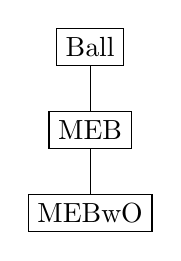
\begin{tikzpicture}
        \Tree [
            .\node[draw]{Ball}; [
                .\node[draw]{MEB}; [
                    .\node[draw]{MEBwO};
                ]
            ]
        ]
    \end{tikzpicture}
    \caption{Class Hierarchy}
    \label{fig:hierarchy}
\end{figure}

These objects have attributes such as a centre and radius and allow us to define an MEB or MEBwO as a single variable as an instance of their corresponding object, which allows for more streamlined implementation, as opposed to tracking values such as the center and radius within seperate, unrelated variables. These objects also implement methods such as \texttt{.fit()} which, given a data input and a chosen method and relevant parameters, will solve the MEB or MEBwO problem on that data set. Other methods are implemented and the reader may refer to the aforementioned \texttt{ball.py} module for a comprehensive guide. All other modules within this package are used by \texttt{ball.py} and are simply used to abstract methods out of this module so as to adhere to good programming principles. Our exact models are formulated and solved using Gurobi in \texttt{gurobi\_solvers.py}.

The \texttt{data} package contains modules regarding the data used in this paper. The \texttt{generation.py} module contains functions which generate each type of data set described in Section \ref{data}, as well as some others which were used in the testing and development of our methods but are not mentioned further within this paper. \texttt{loading.py} contains a few utility functions regarding loading and saving data in a consistent way for ease of implementation. \texttt{benchmarking\_data.py} can be run to generate the data used in our benchmarking, and must be run if the reader wishes to obtain our data as the data sets generated are cumulatively too large to reasonably be uploaded to Github.

The \texttt{benchmarking} package contains the \texttt{trials.py} module which contains functions used for benchmarking, though the code in here is not very good from a software engineering perspective so I will neglect to detail it further. The other module in this package, \texttt{utils.py}, simply abstracts various functions away from \texttt{trials.py}.

\section{Data}\label{data}
In this section we present and discuss the types of data we will use for bench-marking our algorithms for solving the MEBwO problem. Functions written and used for this project can be found in the module \texttt{src/data/generation.py}.

\subsubsection{On Random Number Generation}
In order to generate our data, we must have some method of creating random numbers. To generate uniform random variates from the distribution $U(0,1)$, the method of linear congruential generators \cite{lcg1,lcg2} is well known within the literature, and provide us a computationally trivial way of generating pseudo-random uniform numbers.

With a source of pseudo-random uniform numbers, it is then possible to create a wide variety of different random variates from various distributions. For example, to sample a random variate from the distribution $U(a,b)$ where $a>b$, one must simply generate a random variate $U$, from the distribution $U(0,1)$, then $U(b-a)+a$ follows the distribution $U(a,b)$. To generate standard normal random variates from uniform random variates, one can use methods such as the Box-Muller transform \cite{boxmuller}.

Using linear congruential generators and then applying transformations to obtain other random variates allows the user direct control over the randomness in their computations, allowing for very easy reproducability. In our implementation, we instead use the \texttt{random} package from NumPy \cite{numpy}. This allows us to generate uniform random numbers using \texttt{np.random.uniform} and \texttt{np.random.normal} easily, and we may set a seed for the pseudo-random generator using \texttt{np.random.seed} for reproducability.


\subsection{Normal}
Our first data set is constructed by generating standard normal variates, that is random numbers from the normal distribution $X\sim N(0,1)$ with mean $0$ and variance $1$. Many examples of real-life data have been shown to be normally distributed and the normal distribution is symmetric around its mean in each dimension, so it is an obvious choice to be fit with an MEBwO.

This can be easily generated using NumPy \cite{numpy} by calling the function \texttt{np.random.normal(0, 1, (n,d))} to generate $n$ many $d$-dimensional standard normal vectors. See Figure \ref{fig:normal} for an example.

\datafigure{normal}{Example of Standard Normal Data}{fig:normal}

\subsection{Uniform Ball}\label{uniform ball}
Our next data type consists of points sampled uniformly from a hypersphere of dimension $d$, and in this paper we will specifically choose to uniformly sample points within the unit ball centered on the zero vector, $B(\mathbf{0},1)\subseteq\mathbb{R}^d$. See Figure \ref{fig:unifball} for an example. Like with the choice of normal data, spherical data such as that of a uniform ball is a reasonable choice for the MEBwO problem.

\datafigure{uniform_ball}{Example of a Uniform Ball}{fig:unifball}
%TODO: 3d looks a bit squished
To generate points uniformly within a unit ball, we must first generate points uniformly on the unit hypersphere. \cite{hyperspheresurface} provides a fast and easy to implement method of doing this, by first generating the standard normal vector $\mathbf{x}=(x_1,\ldots,x_d)$ where $x_i\sim N(0,1)$ for $i=1,\ldots,d$, and then the distribution of the normalized vectors $\mathbf{x}/\norm{\mathbf{x}}$ is uniform over the hypersphere of dimension $d$.

A naive approach would then be to multiply the point on the surface of the hypersphere by a uniform random variate $U\sim U(0,1)$ to obtain a point inside the unit ball, and indeed this does generate points within the unit ball, but they will not be uniformly distributed and points will be more densely located near the centre of the ball. Instead, from \cite{eldredge} we find that we can instead multiply our point on the surface of the hypersphere by $U^{1/d}$ to have our points be uniformly distributed within the hypersphere. More generally, multiplying our point on the surface by $r\cdot U^{1/d}$ for some radius $r>0$ gives us a point within the hypersphere of radius $r$. See Algorithm \ref{alg:unitball} for a detailed outline of this method.

\begin{algorithm}[H]
    \KwIn{Dimension $d\in\mathbb{N}$, radius $r\in\mathbb{R}^{\geq0}$, centre $c\in\mathbb{R}^d$}
    \KwOut{Point $x\in\mathbb{R}^d$}
    Generate $x:=(x_1,\ldots,x_d)$ where $x_i\sim N(0,1)$\;
    $x:=x/\norm{x}$\;
    Generate $U\sim U(0,1)$\;
    $x:=r\cdot x\cdot \left(U^{1/d}\right)$\;
    $x:= x+c$\;
    \KwRet{x}
    
    \caption{Algorithm for Generating Points in a Hypersphere of Radius $r$}
    \label{alg:unitball}
\end{algorithm}

One benefit of using this data is that when we are bench-marking the Relaxation-Based Heuristic, we do not need to spend time calculating a lower bound for $M$. Since we know our data set is contained within a unit ball, our diameter can be at most 2. The true diameter of any given uniform ball data set will be some value marginally close to 2, but crucially, less than 2. This means an $M$ value of 2 will ensure that our big $M$ constraints work correctly, and the closeness of the true diameter to 2 means that the increase in solution time for the exact model is negligible.

\subsection{Hyperspherical Shell}
Now we will discuss the data type we call the Hyperspherical Shell. This consists of points sampled uniformly between the surfaces of two concentric hyperspheres with the same centres where one is strictly contained within the other. We may explicitly define this region as
\begin{equation*}
    H(c,r_1,r_2) = \left\{x\in\mathbb{R}^d: r_1 \leq \norm{x-c} \leq r_2\right\}
\end{equation*}

In this paper we choose the zero vector as our center, an inner radius of $1$, and an outer radius of $2$. See Figure \ref{fig:hypshell} for an example. In two dimensions the shape approximated by this data is known as an annulus, and in three dimensions a spherical shell, so for the general $d$-dimensional case we opt to call it a hyperspherical shell.

\datafigure{hyperspherical_shell}{Example of a Hyperspherical Shell}{fig:hypshell}
%TODO: colour code to make 3d plot clearer

This data type is chosen as the optimal centre of the MEBwO on any sufficiently large data set is guaranteed to be ``far" away from any point in the data set. This poses issues for Shenmaier's Approximation which always returns a centre which is a point within the data set.

To generate points within this set, we can make use of Algorithm \ref{alg:unitball} to generate points uniformly in a hypersphere whose radius is our chosen outer radius, then use an acceptance-rejection method to reject points whose distance from our chosen centre is less than our chosen inner radius. A common drawback of acceptance-rejection methods is that of efficiency, i.e. of the space in which we are generating points, what percentage of this space is our acceptance region. Depending on the amount of points desired, a low efficiency can result in very long computation times due to the number of points being rejected.

Acceptance-rejection methods are usually unsuitable for generating high-dimensional data, as a result of the ``curse of dimensionality". For example, if we wanted to generate points within a unit ball using an acceptance-rejection method, the ratio of the volume of a hypersphere inscribed within a hypercube to the volume of that hypercube tends to $0$ as $d\to\infty$ \cite{curse}.

Fortunately, in our case, the ratio of the acceptance region to the total volume of the hypersphere tends to $1$ as $d\to\infty$. To see this, note that the volume of a $d$-dimensional hypersphere with radius $r$ is
\begin{equation*}
    V_d(r) = \frac{S_d r^d}{d}
\end{equation*}
where $S_d$ is the hyper-surface area of the unit hypersphere in $d$ dimensions \cite{hypersphere}. Now, for inner radius $r_1$ and outer radius $r_2$ where $r_2>r_1$, we have
\begin{align*}
    \frac{V_d(r_1)}{V_d(r_2)} &= \frac{\left(\frac{S_dr_1^d}{d}\right)}{\left(\frac{S_dr_2^d}{d}\right)} \\
    &= \frac{r_1^d}{r_2^d} \\
    &= \left(\frac{r_1}{r_2}\right)^d
\end{align*}
which tends to $0$ as $d\to\infty$ since $r_2>r_1$. So, for sufficiently large $d$, the efficiency of this acceptance-rejection method is close to $1$. We outline our acceptance-rejection method in Algorithm \ref{alg:shell}

\begin{algorithm}
    \KwIn{Dimension $d\in\mathbb{N}$, inner radius $r_1\in\mathbb{R}^{\geq0}$, outer radius $r_2\in\mathbb{R}^{\geq0}$, center $c\in\mathbb{R}^d$}
    \KwOut{Point $x\in\mathbb{R}^d$}
    
    \While{True}{
        Generate $x$ from Algorithm \ref{alg:unitball} with $r=r_2$\;
        \uIf{$\norm{x-c}>r_1$}{
            break\;
        }
    }
    \KwRet{x}\;
    
    \caption{Acceptance-Rejection Method for Generating Points in a Hyperspherical Shell}
    \label{alg:shell}
\end{algorithm}

Like with the Uniform Ball data, Hyperspherical Shell data will have a guaranteed upper bound to the diameter and so we will not need to calculate $M$.
\subsection{Uniform Ball with Outliers}
Our final randomly generated data set is the Uniform Ball with Outliers. This data type consists of a uniform ball with a set amount of ``outliers" which we generate ourselves. The main benefit of using this data type to benchmark our algorithms is that since we can choose the exact number of points outside the uniform ball, if we set $\eta\%$ of our $n$ points to be outside of the ball with radius $r$ then $\MEBwO(\A,\eta)$ will have a radius close to $r$.

To generate this data, we simply use Algorithm \ref{alg:unitball} to generate a uniform unit ball with radius $1$ which contains $\eta\%$ of our data, and then use Algorithm \ref{alg:shell} with inner radius $2$ and outer radius $3$ which contains $(1-\eta)\%$ of our data. We choose an inner radius of $2$ so that there is a distinct gap between the two parts of the data in the interest of having a clear inner ball. See Figure \ref{fig:unifballoutliers} for an example. Like before, we do not need to calculate an $M$ value for this data as we have a guaranteed upper bound to the diameter.

\begin{algorithm}
    \KwIn{Number of points $n\in\mathbb{N}$, dimension $d\in\mathbb{N}$, percentage of inliers $\eta\in\left[0,1\right]$, radius of ball $r\in\mathbb{R}^{\geq0}$, inner radius of shell $r_1\in\mathbb{R}^{\geq0}$, outer radius of shell $r_2\in\mathbb{R}^{\geq0}$}
    \KwOut{Data set $\A\subseteq\mathbb{R}^d$}
    
    $n_1:=\floor{\eta\cdot n}$\;
    $n_2:=\floor{(1-\eta)n}$\;
    Let $\A_1$ be the data set generated by running Algorithm \ref{alg:unitball} $n_1$ many times for $r=r$\;
    Let $\A_2$ be the data set generated by running Algorithm \ref{alg:shell} $n_2$ many times for $r_1=r_1$, $r_2=r_2$\;
    $\A:=\A_1\cup\A_2$\;
    \KwRet{$\A$}
    
    \caption{Algorithm for Generating a Uniform Ball with Outliers}
    \label{alg:unifballoutliers}
\end{algorithm}

\datafigure{uniform_ball_with_outliers}{Example of a Uniform Ball with Outliers}{fig:unifballoutliers}


\subsection{MNIST}

In the interest of easy reproducability and an example of a real-life application, we would like to test our construction methods on the MNIST data set \cite{lecun2010mnist}. This data set consists of 70000 hand-written digits from 0--9 which are size-normalized and centered in $28\times28$ pixel greyscale images, and examples can be seen in Figure \ref{fig:mnist_example}. MNIST is a popular data set for testing digit recognition models, a specific application of the broader class of image recognition models within computer vision. We may fit an MEBwO to the subset of data for a specific digit and this ball may then be used for outlier recognition or as a more robust binary classification model than if one were to use an MEB. Further to this, seperate balls may be fit to each digit and used to make multi-class classifications, either in a voting-based ensemble model or as part of a decision tree. In Section (TODO: REF OUTLIER RECOGNITION) we will apply two of our algorithms as an outlier recognition method.

\begin{figure}
    \centering
    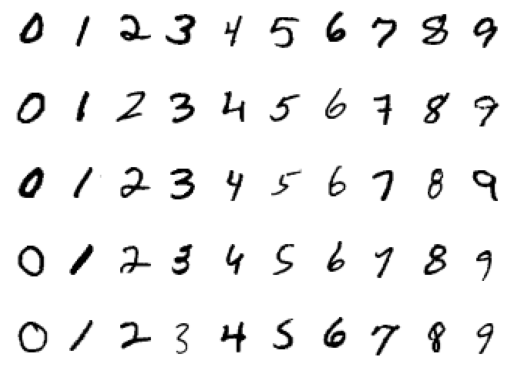
\includegraphics[width=0.5\textwidth]{mnist_example.png}
    \caption{Example of MNIST Data}
    \label{fig:mnist_example}
\end{figure}

In order to make this data usable by our algorithms, we would like to express each image as a vector. To do this we may simply transform each pixel value (an integer in the range 0--255) to an element of a $784$-dimensional array, and this is easily achieved using the \texttt{np.ndarray.flatten} method from NumPy.

\chapter{Experiments}
In this chapter we present our experimental results from applying our algorithms to different types of data. For each class of benchmarks we first discuss the methodology used to gain results and then present and discuss those results.

As discussed in Section \ref{sec:software} we implement our algorithms in Python 3.8. Results were obtained on a HP ENVY x360-15-dr0005na\footnote{\url{https://support.hp.com/gb-en/document/c06378310}} laptop running Ubuntu 20.04.2 LTS, with an Intel(R) Core(TM) i7 8565U  processor and 16GB DDR4-2400 SDRAM.


\section{Exact Model}\label{exact benchmarks}
\subsection{Methodology}
Our interest in benchmarking the exact solver is simply to demonstrate the impracticality of using it to solve any reasonably sized problems, rather than an assessment of how this method is able to solve different types of problems. So, in order to save time, we benchmark the solver just on normal data.

Parameters chosen for $n$ were $n=300$ to $n=750$ in steps of 50 with $d=10$ and $\eta=0.9$ fixed. For $d$ we choose $d=2$ to $d=20$ in steps of 2 with $n=300$ and $\eta=0.9$ fixed, and for $\eta$ we choose $\eta=0.5$ to $\eta=1$ in steps of 0.05 with $n=300$ and $d=10$ fixed. Note that the $\eta=1$ case reduces to the standard MEB problem.

In Section \ref{sec:M} we discussed the effects of the big $M$ parameter on the solution time of the solver, and so we also benchmark the solutuon time when this parameter is varied. To calculate a lower bound on $M$ which ensures that our constraints work as intended, we use the maximum pairwise distance as discussed in the aforementioned section. This is a suitable choice as the size of data sets we use to benchmark the solver are relatively small and so calculating each pairwise distance does not take too much time. Then, we solve the model on the same data set while increasing $M$ in steps of $M/2$.

We generate a large data set ($1000\times100000$) of random normal variates, from which we may sample $n$ many $d$-dimensional vectors to use as a data set. For each choice of parameters, we solve 5 different models and record details such as the center and radius, elapsed time from the solver, and more to a log file. While we choose 5 for our number of trials, more is always better in this context but due to the time constraints of the project we deemed 5 to be a sufficient amount of trials. In presenting our results we give the average elapsed time, though exact times for each solved instance may be found in the log files in the \texttt{benchmarks} folder in the Github repository.

\subsection{Results}
\begin{figure}[ht]
    \centering
    \begin{subfigure}[b]{0.475\textwidth}
        \centering
        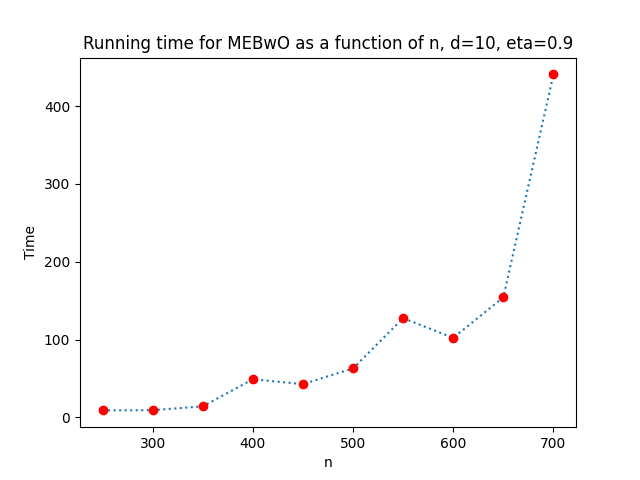
\includegraphics[width=\textwidth]{exact_benchmarks/func_n_d10_eta0p9_normal.png}
        \caption{By $n$}
        \label{fig:exact_benchmarks_n}
    \end{subfigure}
    \hfill
    \begin{subfigure}[b]{0.475\textwidth}
        \centering
        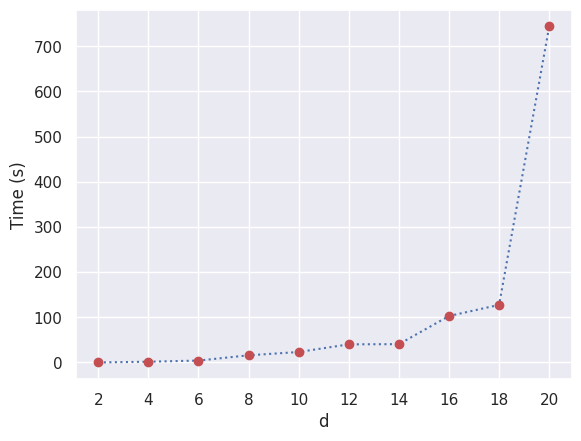
\includegraphics[width=\textwidth]{exact_benchmarks/func_d_n300_eta0p9_normal.png}
        \caption{By $d$}
        \label{fig:exact_benchmarks_d}
    \end{subfigure}
    \hfill
    \begin{subfigure}[b]{0.475\textwidth}
        \centering
        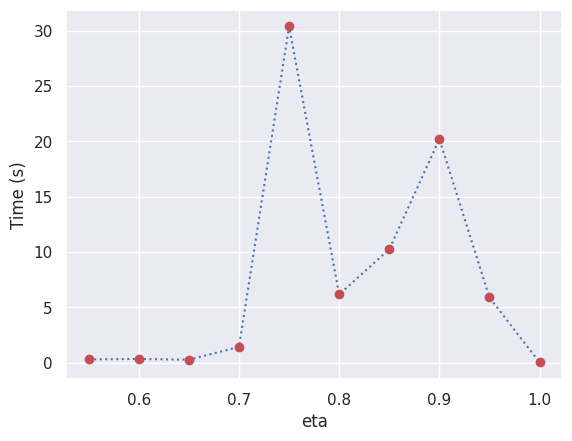
\includegraphics[width=\textwidth]{exact_benchmarks/func_eta_n300_d10_normal.png}
        \caption{By $\eta$}
        \label{fig:exact_benchmarks_eta}
    \end{subfigure}
    \hfill
    \begin{subfigure}[b]{0.475\textwidth}
        \centering
        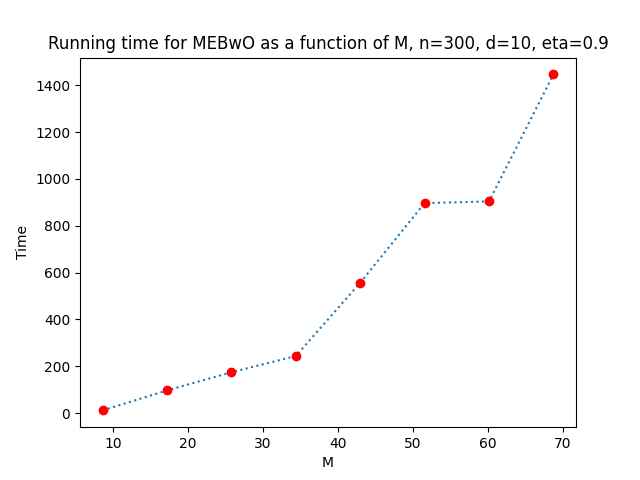
\includegraphics[width=\textwidth]{exact_benchmarks/func_M_n300_d10_eta0p9_normal.png}
        \caption{By $M$}
        \label{fig:exact_benchmarks_M}
    \end{subfigure}
    \caption{Runtimes for the Exact Model on Normal Data}
    \label{fig:exact_benchmarks}
\end{figure}
% TODO: add more detail to captions (specify fixed parameters)
In Figure \ref{fig:exact_benchmarks_n} and Figure \ref{fig:exact_benchmarks_d} we observe gradual increases in runtime as each parameter increases, until we see a sharp increase in runtime. This is what we expected due to the highly combinatorial nature of this problem, though we did not expect such a large and sudden change. One potential explanation to this is optimizations made by the Gurobi solver which make smaller instances quicker to solve, but eventually lose effedctiveness as problem size increases. These optimizations are how Gurobi Optimization make their money and are not publicly known so we are not able to comment on exactly how they achieve this.

Figure \ref{fig:exact_benchmarks_eta} also produces strange results, as we would expect the maximum number of feasible solutions to be available when $\eta=0.5$, but the solver is actually able to solve these instances from 0.5 up to 0.7 extremely quickly. We observe spikes at $\eta=0.75$ and $\eta=0.9$, and again the exact behaviour we observe here is hard to explain due to the closed nature of the Gurobi solver.

Figure \ref{fig:exact_benchmarks_M} shows exactly what we expect, which is increasing runtime as $M$ increases beyond what is necessary. This provides justification for some sort of optimized approach to calculating a lower bound as we have done in order to reduce run times as discussed in Section \ref{sec:M}.


\section{Construction Methods}
\subsection{Methodology}
To benchmark our construction methods we take a similar approach to that of benchmarking the exact model. We generate separate data sets of each type for a given set of parameters, so that each method is benchmarked on exactly the same data sets.

For benchmarking $n$ we choose $n=1000$ to $n=28000$ in steps of 3000 with $d=30$ and $\eta=0.9$ fixed. For $d$ we choose $d=10$ to $d=100$ in steps of 10 with $n=10000$ and $\eta=0.9$ fixed. For $\eta$ we choose $\eta=0.5$ to $\eta=0.9$ in steps of 0.1 with $n=10000$, $d=30$ fixed.

Like with the exact model, we solve the MEBwO problem with our methods on 5 different data sets for each choice of parameters, and again would prefer to do more but we chose 5 due to the time restrictions. Each solved instance has its solutions, runtime and other details recorded to a log file. Runtime is recorded using Python's \texttt{timeit} library, calling the timer before and after running each algorithm. When we use the Relaxation-Based Heuristic, we calculate a lower bound for the $M$ value required to solve the relaxed model by solving the MEB problem and setting $M:=2r$ where $r$ is the solution for the radius of the MEB problem, as discussed in Section \ref{sec:M}. This is only actually necessary for the normal data, as each of the other data types has a maximum diameter determined by the parameters chosen to generate it (see Section \ref{data}).

In presenting our results, we again report average radii and runtimes while exact solutions and runtimes are available in the log files in the \texttt{benchmarks} folder in the Github repository and tabular results may be found in the Appendix \ref{app:constr_tables}. We provide graphs which group results by data type and algorithm, so one may compare the performance of each algorithm on one data type as well as the performance of one algorithm on each data type. When grouping by data type we also present the radii returned by each method so we may compare the radii returned by each method on the same data, while it does not make sense to compare radii returned by one algorithm on different data types. Note that in some plots, some methods are not visible, but this is because they is covered by the markers for other methods when they give the same solutions. We do not report runtime for the average point heuristic as this runs extremely quickly, but runtime plots are given separately in Appendix \ref{app:aph_runtime} for completeness. When grouping by function we are interested in how the runtime varies so that we may verify our time complexity derivations and do not report solutions.

\subsection{Results}
\subsubsection{By Data Type}
%TODO: want to put figures close to the text that talks about them
\benchmarkfiguresix{normal}{Normal}
On normal data we observe that Shenmaier's approximation gives strictly worse solutions as both $n$ and $d$ vary. For $n$ Shenmaier's approximation also has the longest run time for each $n$, while for $d$ it runs in less time than the relaxation-based heuristic for $d$ greater than 50. The average point heuristic tends to perform the best on normal data while also sporting near-instant runtimes.

\benchmarkfiguresix{uniform_ball}{Uniform Ball}
On uniform ball data, the relaxation-based heuristic and shrink heuristic give the same solutions as each parameter varies, but the shrink heuristic has strictly shorter runtimes for each parameter. The average point heuristic also gives the same solutions with insignificant runtimes. Shenmaier's approximation has shorter runtimes for $d$ greater than 70, but has significantly worse radii on these instances (around 40\% worse).


\benchmarkfiguresix{hyperspherical_shell}{Hyperspherical Shell}
On hyperspherical shell data we observe a similar story to that of uniform ball data, with the relaxation-based heuristic, shrink heuristic, and average point heuristic again giving the same results, with the shrink heuristic running in less time than the relaxation-based heuristic for each parameter. Shenmaier's approximation again is the fastest method for $d$ greater than 70, but like before has strictly worse performance.


\benchmarkfiguresix{uniform_ball_with_outliers}{Uniform Ball with Outliers}
On uniform ball with outliers data, the relaxation-based heuristic is our best performing method, though we observe a larger than usual increase in runtime as the dimension increases, with a runtime of a little over an hour for each instance at $d=80$, so we were unable to solve instances for $d=90$ and $d=100$ within the time constraints. The shrink heuristic as usual gives short runtimes with only marginally worse radii, though also marginally worse radii than the average point heuristic for small $n$. Each of these methods have very similar solutions for large $n$ and all $d$. Recall that the optimal solution for our uniform ball with outliers data will be a radius of 1, which is indeed returned by the relaxation-based heuristic while the shrink heuristic returns radii marginally above 1. Shenmaier's approximation gives far worse than expected solutions, on average around 55\% worse than optimal.


\subsubsection{By Algorithm}
\benchmarkfigurebyfunc{relaxation_heuristic}{Runtimes for Relaxation-Based Heuristic on each Data Type}{fig:rbh_benchmarks}
The complexity of the relaxation-based heuristic is hard to assess due to being solved by an optimization solver, so these plots are able to give us some insight. With respect to $n$, we can observe a trend somewhere between linear and polynomial. With respect to $d$, the trend appears to be polynomial, and with respect to $\eta$ there does not appear to be any strong trend.

\benchmarkfigurebyfunc{shenmaier}{Runtimes for Shenmaier's Approximation on each Data Type}{fig:shenmaier_benchmarks}
We know that the average time complexity of Shenmaier's approximation will be $O(n^2d)$ which is fortunately exactly what we observe in these plots. We would expect no significant difference in runtimes when comparing data types since Shenmaier's approximation works by iterating over each point, but we do see slight differences in runtime then varying the dimension of the data. This could be explained by the sorting of distances which takes place when finding the $k$ closest points, as this list will have a different distribution when sorted for each data type. The overall trend as dimension is increased is linear but we observe a lesser increase in runtime than expected. This is likely because of optimizations made by NumPy where the computations for arrays/vectors are written in C.


\benchmarkfigurebyfunc{shrink}{Runtimes for Shrink Heuristic on each Data Type}{fig:shrink_benchmarks}
Recall that the shrink heuristic's time complexity depends on the algorithm used to solve the initial MEB problem, which in our implementation is Algorithm \ref{core-set algorithm} from \cite{core-sets} with time complexity $O\left(\frac{nd}{\epsilon}+\frac{d^2}{\epsilon^{3/2}}\left(\frac{1}{\epsilon}+d\right)\log\frac{1}{\epsilon}\right)$. We indeed see a linear relationship between runtime and $n$ and a polynomial relationship between runtime and $d$. Interestingly we have almost no relationship between runtime and $d$ for normal data, and the reason for this is unclear. There is no relationship observed between runtime and $\eta$ as expected, except for uniform ball with outliers data, which makes sense considering the structure of the data is dependent on $\eta$ which evidently has an effect on the runtime of this algorithm, which works by finding a core-set for the data which we would assume is easier to find when there are less points in the outer shell.

\section{Improvement Heuristics}
\subsection{Methodology}
Our interest in benchmarking our improvement heuristics is in how well these heuristics improve an existing solution. Runtime is not a concern as we know that both heuristics will terminate very quickly as discussed in Section \ref{sec:improvement_heuristics}, though we include plots of the runtimes for the DCMEB model in the appendix (TODO: REF THIS) for completeness.

These heuristics were designed to be used after gaining a solution from Shenmaier's approximation, so we first find this solution for the given data set and then run an improvement heuristic 100 times. As discussed in Section \ref{sec:improvement_heuristics} other stopping criteria could be implemented but we opt for an iteration limit for ease of implementation and simplicity.

As seen in the previous section, Shenmaier's algorithm is not a particularly fast method, so with regard to the time constraint of this project we choose to benchmark our improvement heuristics on separate, smaller data sets than those we used to benchmark our construction methods. We follow the same methodology in generating and saving each data set. For benchmarking $n$ we choose $n=500$ to $n=5000$ in steps of 500 and for $d$ we choose $d=10$ to $d=150$ in steps of 10. The improvement heuristics, while primarily useful for improving an existing MEBwO, ultimately only improves an MEB on a subset of data so there is no $\eta$ parameter to vary.

In each instance we solve, we record the initial radius returned by Shenmaier's approximation, and after running the improvement heuristic 100 times we record the new improved radius. In the results section we report average improvement for each heuristist, where if $r$ is the initial radius and $\hat{r}$ is the improved radius, the improvement percentage is calculated as $(1-\hat{r}/r)\cdot100$. Tabular results may be found in Appendix \ref{app:impr_tables}.

\subsection{Results}
\subsubsection{DCMEB Runtime}

\begin{figure}[ht]
    \centering
    \begin{subfigure}[b]{0.475\textwidth}
        \centering
        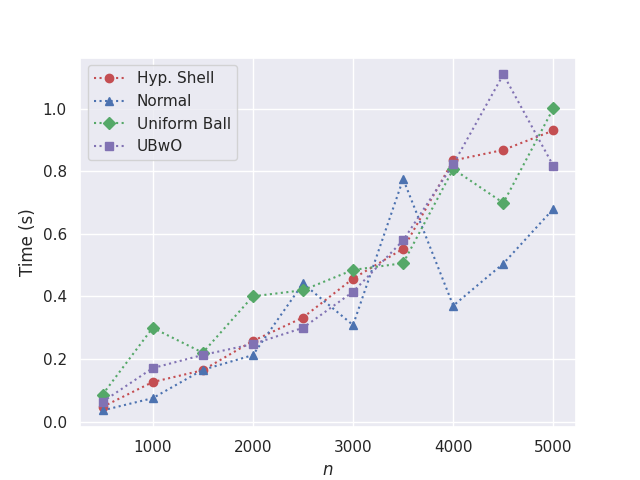
\includegraphics[width=\textwidth]{images/dcmeb_benchmarks/func_n_d100_eta0p9_uniform_ball_with_outliers.png}
        \caption{By $n$}
        \label{fig:dcmeb_plot_n}
    \end{subfigure}
    \hfill
    \begin{subfigure}[b]{0.475\textwidth}
        \centering
        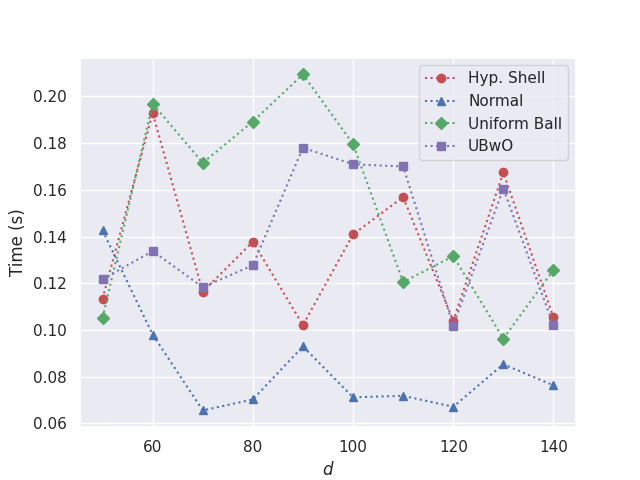
\includegraphics[width=\textwidth]{images/dcmeb_benchmarks/func_d_n1000_eta0p9_uniform_ball_with_outliers.png}
        \caption{By $d$}
        \label{fig:dcmeb_plot_d}
    \end{subfigure}
    \caption{Runtimes for the DCMEB Model on each Data Type}
    \label{fig:dcmeb_plot}
\end{figure}

From these plots we see what looks to be a polynomial relationship between runtime and $n$ as expected when using an interior point method, and no relationship between runtime and $d$. Although the longest that a single model took to solve was about 1.1 seconds, since this model is solved many times (100 in our case) this leads to non-insignificant runtimes when applying the heuristic, especially when compared to the DCSSH which runs in linear time.

\subsubsection{Performance}
\imprfigure{normal}{Average Improvement Performance on Normal Data as a Function of $n$ and $d$}{fig:improvement_normal}

\imprfigure{uniform_ball}{Average Improvement Performance on Uniform Ball Data as a Function of $n$ and $d$}{fig:improvement_unifball}

\imprfigure{hyperspherical_shell}{Average Improvement Performance on Hyperspherical Shell Data as a Function of $n$ and $d$}{fig:improvement_hypshell}

\imprfigure{uniform_ball_with_outliers}{Average Improvement Performance on Uniform Ball with Outliers Data as a Function of $n$ and $d$}{fig:improvement_unifballwoutliers}

From the first three plots we see the same trends, where the average improvement decreases as $n$ decreases and average improvement increases as $d$ increases. This is likely due to more free space between points near the surface of the ball and that surface as dimension increases, while increasing the number of points will mean there are more points which are near the surface, thus giving a lower minimal distance between each point and the surface of the ball in the opposite improving direction. Interestingly we observe the exact opposite trend for the uniform ball with outliers data and it is uncertain why this is, though it is likely due to the unique structure of this data type.

Both heuristics give very similar performances, though the DCSSH appears to always be marginally better than the DCMEB. We can then conclude that, out of these two heuristics, one should always use the DCSSH over the DCMEB since the DCSSH runs in linear time as opposed to the polynomial time of the DCMEB, and for ease of implementation as the DCSSH does not require the use of an optimization solver which requires specific knowledge of how to use and in a commercial setting will in most cases require a payment of sorts.

\section{Outlier Recognition}
\subsection{Methodology}
We largely follow the methodology in \cite[Section 4.2]{huding} by Hu Ding and Mingquan Ye for benchmarking their algorithm on the MNIST data set. For each digit 0--9, we construct a base data set by taking all points corresponding to that digit, then randomly sample points from the remaining digits as outliers. So, suppose we have $n$ many points which are labelled 0, we then sample $(1-\eta)n$ many outliers from the digits 1--9. We use the entire 70000-point data set for this as we are not interested in a test-train split for an outlier recognition problem.

Once we have solved each instance, to measure the performance of the MEBwO as an outlier recognition model we calculate the $F_1$ score which is defined as
\begin{equation*}
    F_1 = 2\cdot\frac{\text{Precision}\cdot\text{Recall}}{\text{Precision}+\text{Recall}}
\end{equation*}
where the precision and recall are defined as 
\begin{equation*}
    \text{Precision} = \frac{\text{TP}}{\text{TP} + \text{FP}},\quad \text{Recall} = \frac{\text{TP}}{\text{TP}+\text{FN}}
\end{equation*}
and $\text{TP}$, $\text{FP}$, and $\text{FN}$ are the number of true positives, false positives, and false negatives respectively found by the model. In our context, true positives are points which are inside the ball and are the desired digit, false positives are points which are inside the ball and are not the desired digit, and false negatives are points which are outside the ball and are the desired digit. The $F_1$ score is a common metric used to assess binary classification models such as outlier recognition models, and varies from 0 to 1 with an $F_1$ score of 1 indicating perfect performance.

For each method and each parameter we solve the MEBwO problem for each digit and then report the average $F_1$ score across each digit. Due to the random sampling in constructing each instance we would prefer to report average performance for each digit across multiple instances, but due to time constraints this is not possible and we hope that averaging across each digit provides enough robustness to the issues associated with random sampling.

The algorithm in \cite{huding} is compared against three outlier recognition methods, which are angle-based outlier detection (ABOD) \cite{abod}, one-class support vector machine (OCSVM) \cite{ocsvm}, and discriminative reconstructions in an auto-encoder (DRAE) \cite{drae}. See \cite{huding} for further details. We provide an extension to Table 2 of this paper, referring to their algorithm as HDMY. The total time reported is the total running time for each value of $\eta$ and we assume this is averaged over each of their 20 instances. It should be noted that the time for sampling is included in the runtimes in their paper, which we do not do, but in our experiments we find this takes at most a few seconds so the effect on the results is negligible considering the total runtime for each algorithm is reported on the order of hours. %TODO: different computer too
%TODO: legend blocks plot in 5.2.1a
We present our results in tabular form as in \cite{huding} but also provide the results as a plot for the reader's enjoyment. It should be noted that HDMY and each of our algorithms are all MEBwO models and we are comparing the effectiveness and runtime of each algorithm used to create the MEBwO. Unfortunately Gurobi was unable to solve the relaxed model required for the relaxation-based heuristic, reaching the memory limit on our machine (16GB) before the model could be instantiated.

\subsection{Results}

\begin{figure}[ht]
    \centering
    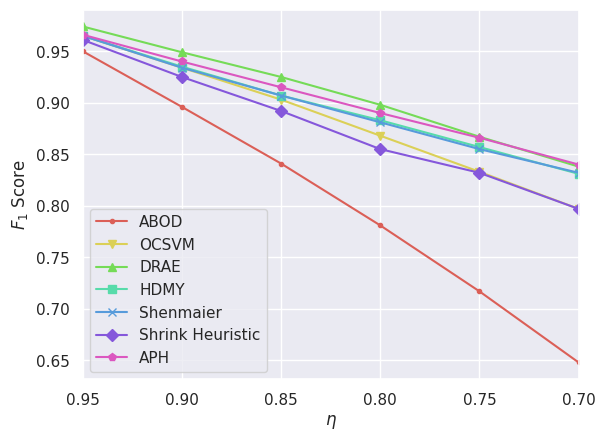
\includegraphics[width=0.6666\textwidth]{images/mnist_plot.png}
    \caption{$F_1$ Score and Runtime of each Method for MNIST Outlier Recognition}
    \label{fig:mnist_fig}
\end{figure}
\begin{table}[ht]
    \centering
    \begin{tabular}{|c||c|c|c|c||c|c|c|} \hline
        $\eta$&ABOD&OCSVM&DRAE&HDMY&Shenmaier&Shrink Heuristic&APH \\ \hline
        0.95&0.95&0.965&0.974&0.965&0.965&0.961&0.966 \\
        0.9&0.896&0.934&0.949&0.935&0.934&0.925&0.94 \\
        0.85&0.841&0.903&0.925&0.907&0.907&0.892&0.915 \\
        0.8&0.781&0.868&0.898&0.883&0.881&0.855&0.89 \\
        0.75&0.717&0.833&0.867&0.857&0.855&0.832&0.866 \\
        0.7&0.648&0.797&0.838&0.831&0.832&0.797&0.84 \\ \hline
        Runtime (s) & $2\times10^4$ & $3.4\times10^3$ & $1\times10^5$ & $1.6\times10^4$ & $5.1\times10^4$ & $1.6\times10^4$ & $131.7$ \\ \hline
    \end{tabular}
    \caption{$F_1$ Score and Runtime of each Method for MNIST Outlier Recognition}
    \label{tab:mnist_table}
\end{table}

Comparing just our algorithms, both Shenmaier's approximation and the average point heuristic achieve similar performance, interestingly with the average point heuristic being marginally better---a surprise to be sure, but a welcome one, considering the very short runtime of the average point heuristic (two minutes compared to fourteen hours). The shrink heuristic finds worse performance than each of our other algorithms despite taking four hours in total to run.

Each of our algorithms is able to outperform the ABOD model and all but the shrink heuristic outperform the OCSVM model. Each algorithm gives worse performance then the DRAE model, which was also true for the algorithm in \cite{huding}. This algorithm gives similar performance to Shenmaier's approximation, but Shenmaier's approximation takes a little over three times as long to run. The average point heuristic is able to outperform HDMY which again is interesting considering the short runtime. It should again be noted that we were unable to run averages for these scores over multiple samplings of the MNIST data set, so it is possible that the average point heuristic on average has a worse performance than in our results, and we have randomly sampled a more favourable set of instances for this algorithm.


% =============================================================================
% Chapter 5
% =============================================================================
\chapter{Conclusion}

% =============================================================================
%the entries have to be in the file literature.bib
\bibliography{literature}
%\addcontentsline{toc}{chapter}{Bibliography}

\clearpage

\begin{appendices}
    \section{Average Point Heuristic Runtime Plots}\label{app:aph_runtime}
    Here we present the runtime plots for the average point heuristic. Since this heuristic has a time complexity of $O(nd\log n)$ we know it will run extremely quickly, and so the runtimes were not included in the main text but we include them here for completeness.
    
    \benchmarkfigurebyfunc{shrink_avg}{Runtimes for the Average Point Heuristic on each Data Type}{fig:aph_benchmarks}
    
    \clearpage
    
    \section{Construction Method Tables}\label{app:constr_tables}
    Here we present all average results for each method, parameter, and data type in tabular form. In order to fit the tables within the page width, values were rounded to two decimal places and method names in the column headers were shortened. For each individual result rather than rounded averages, please refer to the \texttt{benchmarks} folder in the Github repository\footnote{\url{https://github.com/tomholmes19/Minimum-Enclosing-Balls-with-Outliers} \cite{Holmes_Minimum_Enclosing_Balls_2021}}.
    
    The tables are organised by data type, and each table contains results for a single varied parameter, with each pair of columns the radius and runtime for each method. Runtimes are given in seconds.
    
    \subsection{Normal}
    \begin{table}[ht]
        \centering
        \begin{tabular}{|c||c|c||c|c||c|c||c|c|}\hline
            $n$&RBH $r$&RBH $t$&Shenm. $r$&Shenm. $t$&Shrink $r$&Shrink $t$&APH $r$&APH $t$ \\ \hline
            1000&6.37&12.4&7.34&5.38&6.52&0.37&6.32&0.02 \\
            4000&6.54&58.21&7.33&85.02&6.54&0.86&6.35&0.07 \\
            7000&6.75&127.11&7.29&262.29&6.57&1.25&6.35&0.11 \\
            10000&6.74&335.94&7.2&541.61&6.5&1.84&6.34&0.16 \\
            13000&6.84&509.54&7.19&932.43&6.51&2.31&6.35&0.2 \\
            16000&6.89&546.73&7.21&1403.68&6.49&3.17&6.34&0.24 \\
            19000&6.86&726.53&7.18&1978.03&6.5&3.49&6.35&0.29 \\
            22000&6.96&973.81&7.12&2664.51&6.48&3.97&6.34&0.33 \\
            25000&6.93&1637.88&---&---&6.47&4.61&6.34&0.36 \\
            28000&6.94&1774.19&---&---&6.46&5.26&6.35&0.39 \\ \hline
        \end{tabular}
        \caption{Results as a Function of $n$ for each Algorithm on Normal Data}
        \label{tab:normal_table_n}
    \end{table}
    
    \begin{table}[ht]
        \centering
        \begin{tabular}{|c||c|c||c|c||c|c||c|c|} \hline
            $d$&RBH $r$&RBH $t$&Shenm. $r$&Shenm. $t$&Shrink $r$&Shrink $t$&APH $r$&APH $t$ \\ \hline
            10&4.58&26.2&4.11&544.15&4.12&0.99&3.99&0.09 \\
            20&5.79&139.09&5.81&553.07&5.48&1.52&5.33&0.12 \\
            30&6.74&479.08&7.2&553.84&6.5&1.91&6.34&0.15 \\
            40&7.56&487.73&8.3&558.3&7.39&2.89&7.2&0.17 \\
            50&8.21&555.81&9.41&573.78&8.09&3.1&7.95&0.21 \\
            60&8.87&1086.75&10.27&573.47&8.81&4.79&8.62&0.24 \\
            70&9.46&1419.23&11.22&583.22&9.44&6.45&9.26&0.28 \\
            80&10.04&1122.77&11.99&580.02&10.04&7.95&9.83&0.3 \\
            90&10.51&1783.04&12.78&591.72&10.53&15.29&10.37&0.33 \\
            100&11.08&3902.45&13.42&592.52&11.07&28.02&10.88&0.36 \\ \hline
        \end{tabular}
        \caption{Results as a Function of $d$ for each Algorithm on Normal Data}
        \label{tab:normal_table_d}
    \end{table}
    
    \begin{table}[ht]
        \centering
        \begin{tabular}{|c||c|c||c|c||c|c||c|c|} \hline
            $\eta$&RBH $r$&RBH $t$&Shenm. $r$&Shenm. $t$&Shrink $r$&Shrink $t$&APH $r$&APH $t$ \\ \hline
            0.5&7.1&316.75&6.17&530.9&5.55&1.98&5.41&0.15 \\
            0.6&6.88&589.73&6.36&535.7&5.74&1.97&5.59&0.15 \\
            0.7&6.65&253.06&6.58&541.77&5.93&1.98&5.78&0.15 \\
            0.8&6.52&353.67&6.84&545.55&6.16&1.99&6.01&0.15 \\
            0.9&6.74&361.1&7.2&549.43&6.5&1.99&6.34&0.15 \\ \hline
        \end{tabular}
        \caption{Results as a Function of $\eta$ for each Algorithm on Normal Data}
        \label{tab:normal_table_eta}
    \end{table}
    \clearpage
    
    
    \subsection{Uniform Ball}
    \begin{table}[ht]
        \centering
        \begin{tabular}{|c||c|c||c|c||c|c||c|c|}\hline
            $n$&RBH $r$&RBH $t$&Shenm. $r$&Shenm. $t$&Shrink $r$&Shrink $t$&APH $r$&APH $t$ \\ \hline
            1000&1.0&8.04&1.39&4.84&1.0&8.37&1.0&0.02 \\
            4000&1.0&32.25&1.37&84.61&1.0&15.76&1.0&0.05 \\
            7000&1.0&62.13&1.34&262.36&1.0&20.5&1.0&0.09 \\
            10000&1.0&92.07&1.34&536.42&1.0&19.87&1.0&0.13 \\
            13000&1.0&128.33&1.34&912.68&1.0&25.44&1.0&0.17 \\
            16000&1.0&168.09&1.34&1379.14&1.0&29.18&1.0&0.21 \\
            19000&1.0&231.08&1.34&1957.49&1.0&28.08&1.0&0.26 \\
            22000&1.0&310.96&1.34&2618.51&1.0&31.3&1.0&0.28 \\
            25000&1.0&492.28&---&---&1.0&32.89&1.0&0.32 \\
            28000&1.0&466.8&---&---&1.0&33.54&1.0&0.36 \\ \hline
        \end{tabular}
        \caption{Results as a Function of $n$ for each Algorithm on Uniform Ball Data}
        \label{tab:uniform_ball_table_n}
    \end{table}
    
    \begin{table}[ht]
        \centering
        \begin{tabular}{|c||c|c||c|c||c|c||c|c|} \hline
            $d$&RBH $r$&RBH $t$&Shenm. $r$&Shenm. $t$&Shrink $r$&Shrink $t$&APH $r$&APH $t$ \\ \hline
            10&0.99&11.42&1.14&530.74&0.99&2.08&0.99&0.07 \\
            20&0.99&41.34&1.29&576.21&0.99&7.91&0.99&0.1 \\
            30&1.0&93.18&1.34&590.32&1.0&20.88&1.0&0.13 \\
            40&1.0&185.42&1.38&594.8&1.0&58.73&1.0&0.15 \\
            50&1.0&313.6&1.39&601.28&1.0&85.84&1.0&0.18 \\
            60&1.0&572.94&1.4&606.33&1.0&262.42&1.0&0.21 \\
            70&1.0&871.02&1.41&620.63&1.0&494.76&1.0&0.24 \\
            80&1.0&1266.66&1.42&617.78&1.0&770.84&1.0&0.26 \\
            90&1.0&1730.96&1.42&629.06&1.0&1292.3&1.0&0.29 \\
            100&1.0&2689.86&1.43&636.3&1.0&1915.89&1.0&0.32 \\ \hline
        \end{tabular}
        \caption{Results as a Function of $d$ for each Algorithm on Uniform Ball Data}
        \label{tab:uniform_ball_table_d}
    \end{table}
    
    \begin{table}[ht]
        \centering
        \begin{tabular}{|c||c|c||c|c||c|c||c|c|} \hline
            $\eta$&RBH $r$&RBH $t$&Shenm. $r$&Shenm. $t$&Shrink $r$&Shrink $t$&APH $r$&APH $t$ \\ \hline
            0.5&0.98&105.74&1.2&528.0&0.98&20.87&0.98&0.13 \\
            0.6&0.98&73.97&1.23&536.72&0.98&21.25&0.98&0.13 \\
            0.7&0.99&77.04&1.26&538.08&0.99&21.33&0.99&0.13 \\
            0.8&0.99&83.24&1.29&543.65&0.99&21.31&0.99&0.14 \\
            0.9&1.0&93.22&1.34&552.18&1.0&21.27&1.0&0.15 \\ \hline
        \end{tabular}
        \caption{Results as a Function of $\eta$ for each Algorithm on Uniform Ball Data}
        \label{tab:uniform_ball_table_eta}
    \end{table}
    \clearpage
    
    
    \subsection{Hyperspherical Shell}
    \begin{table}[ht]
        \centering
        \begin{tabular}{|c||c|c||c|c||c|c||c|c|}\hline
            $n$&RBH $r$&RBH $t$&Shenm. $r$&Shenm. $t$&Shrink $r$&Shrink $t$&APH $r$&APH $t$ \\ \hline
            1000&1.99&8.61&2.78&5.27&1.99&5.62&1.99&0.02 \\
            4000&1.99&42.17&2.73&85.99&1.99&14.05&1.99&0.07 \\
            7000&1.99&70.81&2.71&266.54&1.99&16.1&1.99&0.11 \\
            10000&1.99&212.18&2.67&544.19&1.99&20.79&1.99&0.15 \\
            13000&1.99&357.39&2.66&917.93&1.99&22.94&1.99&0.19 \\
            16000&1.99&549.89&2.67&1401.93&1.99&28.76&1.99&0.23 \\
            19000&1.99&504.16&2.67&1974.51&1.99&23.89&1.99&0.27 \\
            22000&1.99&616.03&2.67&2660.51&1.99&28.16&1.99&0.31 \\
            25000&1.99&1104.94&---&---&1.99&27.87&1.99&0.35 \\
            28000&1.99&1116.81&---&---&1.99&30.53&1.99&0.39 \\ \hline
        \end{tabular}
        \caption{Results as a Function of $n$ for each Algorithm on Hyperspherical Shell Data}
        \label{tab:hyperspherical_shell_table_n}
    \end{table}
    
    \begin{table}[ht]
        \centering
        \begin{tabular}{|c||c|c||c|c||c|c||c|c|} \hline
            $d$&RBH $r$&RBH $t$&Shenm. $r$&Shenm. $t$&Shrink $r$&Shrink $t$&APH $r$&APH $t$ \\ \hline
            10&1.98&32.05&2.46&531.14&1.98&2.31&1.98&0.09 \\
            20&1.99&108.26&2.59&539.75&1.99&6.62&1.99&0.12 \\
            30&1.99&212.84&2.67&542.96&1.99&21.2&1.99&0.15 \\
            40&1.99&179.66&2.76&544.81&1.99&58.01&1.99&0.17 \\
            50&2.0&317.79&2.79&553.62&2.0&100.81&2.0&0.21 \\
            60&2.0&506.3&2.8&579.88&2.0&249.42&2.0&0.23 \\
            70&2.0&893.33&2.82&613.06&2.0&436.27&2.0&0.27 \\
            80&2.0&1225.61&2.83&609.86&2.0&780.93&2.0&0.29 \\
            90&2.0&1896.26&2.85&621.8&2.0&1174.07&2.0&0.33 \\
            100&2.0&2710.25&2.86&626.08&2.0&1796.83&2.0&0.36 \\ \hline
        \end{tabular}
        \caption{Results as a Function of $d$ for each Algorithm on Hyperspherical Shell Data}
        \label{tab:hyperspherical_shell_table_d}
    \end{table}
    
    \begin{table}[ht]
        \centering
        \begin{tabular}{|c||c|c||c|c||c|c||c|c|} \hline
            $\eta$&RBH $r$&RBH $t$&Shenm. $r$&Shenm. $t$&Shrink $r$&Shrink $t$&APH $r$&APH $t$ \\ \hline
            0.5&1.95&68.28&2.4&566.73&1.95&22.27&1.95&0.15 \\
            0.6&1.97&69.93&2.46&573.75&1.97&22.33&1.97&0.15 \\
            0.7&1.98&80.55&2.52&579.48&1.98&22.28&1.98&0.15 \\
            0.8&1.98&103.16&2.58&579.65&1.99&22.35&1.98&0.15 \\
            0.9&1.99&213.85&2.67&586.54&1.99&22.36&1.99&0.15 \\ \hline
        \end{tabular}
        \caption{Results as a Function of $\eta$ for each Algorithm on Hyperspherical Shell Data}
        \label{tab:hyperspherical_shell_table_eta}
    \end{table}
    \clearpage
    
    
    \subsection{Uniform Ball with Outliers}
    \begin{table}[ht]
        \centering
        \begin{tabular}{|c||c|c||c|c||c|c||c|c|}\hline
            $n$&RBH $r$&RBH $t$&Shenm. $r$&Shenm. $t$&Shrink $r$&Shrink $t$&APH $r$&APH $t$ \\ \hline
            1000&1.0&37.9&1.54&5.8&1.09&1.04&1.02&0.02 \\
            4000&1.0&209.2&1.5&92.97&1.02&3.72&1.01&0.06 \\
            7000&1.0&266.03&1.56&302.46&1.01&6.81&1.01&0.11 \\
            10000&1.0&614.47&1.53&798.67&1.01&9.89&1.01&0.15 \\
            13000&1.0&909.65&1.54&958.93&1.01&12.85&1.01&0.19 \\
            16000&1.0&1146.58&1.55&1525.25&1.0&15.65&1.0&0.23 \\
            19000&1.0&1192.01&1.53&2247.41&1.01&17.79&1.0&0.27 \\
            22000&1.0&1677.9&1.55&3008.78&1.0&19.1&1.0&0.31 \\
            25000&1.0&2400.67&---&---&1.0&24.96&1.0&0.35 \\
            28000&1.0&2797.06&---&---&1.0&24.59&1.0&0.39 \\ \hline
        \end{tabular}
        \caption{Results as a Function of $n$ for each Algorithm on Uniform Ball with Outliers Data}
        \label{tab:uniform_ball_with_outliers_table_n}
    \end{table}
    
    \begin{table}[ht]
        \centering
        \begin{tabular}{|c||c|c||c|c||c|c||c|c|} \hline
$d$&RBH $r$&RBH $t$&Shenm. $r$&Shenm. $t$&Shrink $r$&Shrink $t$&APH $r$&APH $t$ \\ \hline
10&1.0&15.96&1.35&565.55&1.01&1.95&1.01&0.09 \\
20&1.0&221.79&1.51&612.36&1.01&4.01&1.01&0.12 \\
30&1.0&526.7&1.53&625.06&1.01&9.5&1.01&0.15 \\
40&1.0&993.85&1.58&630.42&1.01&18.86&1.01&0.18 \\
50&1.0&1372.71&1.58&640.97&1.01&36.98&1.01&0.22 \\
60&1.0&1771.32&1.57&642.91&1.01&96.25&1.0&0.26 \\
70&1.0&2510.24&1.58&663.83&1.01&156.8&1.0&0.27 \\
80&1.0&4159.73&1.57&653.19&1.01&259.48&1.0&0.29 \\
90&---&---&1.57&670.26&1.01&439.24&1.0&0.33 \\
100&---&---&1.57&678.45&1.01&673.86&1.0&0.38 \\ \hline
        \end{tabular}
        \caption{Results as a Function of $d$ for each Algorithm on Uniform Ball with Outliers Data}
        \label{tab:uniform_ball_with_outliers_table_d}
    \end{table}
    
    \begin{table}[ht]
        \centering
        \begin{tabular}{|c||c|c||c|c||c|c||c|c|} \hline
$\eta$&RBH $r$&RBH $t$&Shenm. $r$&Shenm. $t$&Shrink $r$&Shrink $t$&APH $r$&APH $t$ \\ \hline
0.5&1.0&495.3&1.56&529.62&1.0&16.5&1.01&0.15 \\
0.6&1.09&454.97&1.53&535.17&1.0&15.77&1.01&0.16 \\
0.7&1.0&512.09&1.53&541.98&1.0&15.7&1.01&0.15 \\
0.8&1.0&582.12&1.53&542.77&1.0&13.57&1.01&0.15 \\
0.9&1.0&545.39&1.53&549.27&1.01&10.05&1.01&0.15 \\ \hline
        \end{tabular}
        \caption{Results as a Function of $\eta$ for each Algorithm on Uniform Ball with Outliers Data}
        \label{tab:uniform_ball_with_outliers_table_eta}
    \end{table}

    \clearpage
    
    \section{Improvement Heuristic Tables}\label{app:impr_tables}
    Here we present results for each instance of benchmarking the improvement heuristic. We ran 5 separate instances for each particular benchmark, and $r_i$ represents the initial radius of the $i$th instance returned by Shenmaier's approximation while $\hat{r}_i$ represents the improved radius. The final column is the average improvement percentage which is presented in the main text. Figures are rounded to two decimal places to fit within the page width, and the complete solutions may be found in the Github repository.
    
    \subsection{Normal}
    \begin{table}[ht]
        \centering
        \begin{tabular}{|c||cc||cc||cc||cc||cc||c|} \hline
            $n$&$r_1$&$\hat{r}_1$&$r_2$&$\hat{r}_2$&$r_3$&$\hat{r}_3$&$r_4$&$\hat{r}_4$&$r_5$&$\hat{r}_5$&Avg\% \\ \hline
            500&13.2&12.98&13.92&13.11&13.8&13.3&13.79&13.49&13.62&13.03&3.54 \\
            1000&13.84&13.15&13.75&13.23&13.54&12.81&13.79&13.32&13.7&13.33&4.08 \\
            1500&13.78&13.36&13.5&13.31&13.56&13.21&13.67&13.25&13.72&13.2&2.77 \\
            2000&13.57&13.25&13.49&13.41&13.81&13.33&13.53&13.15&13.5&13.17&2.35 \\
            2500&13.56&12.99&13.51&13.1&13.69&13.09&13.42&13.03&13.71&13.05&3.87 \\
            3000&13.32&13.04&13.6&13.31&13.46&13.08&13.72&13.64&13.6&13.16&2.2 \\
            3500&13.52&13.25&13.61&13.21&13.33&13.03&13.53&13.18&13.35&13.15&2.25 \\
            4000&13.5&13.02&13.55&12.98&13.65&13.21&13.37&13.05&13.64&13.36&3.11 \\
            4500&13.52&13.09&13.61&13.26&13.52&13.24&13.66&13.43&13.69&13.23&2.57 \\
            5000&13.48&13.25&13.49&13.33&13.26&13.01&13.7&13.32&13.06&13.05&1.53 \\ \hline
        \end{tabular}
        \caption{Results as a Function of $n$ for the DCMEB Heuristic on Normal Data}
        \label{tab:normal_dcmeb_table_n}
    \end{table}
    
    \begin{table}[ht]
        \centering
        \begin{tabular}{|c||cc||cc||cc||cc||cc||c|} \hline
            $n$&$r_1$&$\hat{r}_1$&$r_2$&$\hat{r}_2$&$r_3$&$\hat{r}_3$&$r_4$&$\hat{r}_4$&$r_5$&$\hat{r}_5$&Avg\% \\ \hline
            500&13.2&12.98&13.92&13.12&13.8&13.3&13.79&13.51&13.62&13.03&3.5 \\
            1000&13.84&13.15&13.75&13.24&13.54&12.81&13.79&13.33&13.7&13.33&4.05 \\
            1500&13.78&13.36&13.5&13.32&13.56&13.22&13.67&13.26&13.72&13.2&2.73 \\
            2000&13.57&13.26&13.49&13.41&13.81&13.33&13.53&13.15&13.5&13.17&2.33 \\
            2500&13.56&12.99&13.51&13.1&13.69&13.11&13.42&13.05&13.71&13.05&3.82 \\
            3000&13.32&13.05&13.6&13.32&13.46&13.1&13.72&13.64&13.6&13.16&2.14 \\
            3500&13.52&13.25&13.61&13.21&13.33&13.03&13.53&13.19&13.35&13.15&2.22 \\
            4000&13.5&13.02&13.55&12.99&13.65&13.21&13.37&13.05&13.64&13.36&3.09 \\
            4500&13.52&13.09&13.61&13.26&13.52&13.24&13.66&13.43&13.69&13.23&2.57 \\
            5000&13.48&13.25&13.49&13.33&13.26&13.01&13.7&13.32&13.06&13.05&1.53 \\ \hline
        \end{tabular}
        \caption{Results as a Function of $n$ for the DCSSH on Normal Data}
        \label{tab:normal_dcssh_table_n}
    \end{table}
    
    \begin{table}[ht]
        \centering
        \begin{tabular}{|c||cc||cc||cc||cc||cc||c|} \hline
            $d$&$r_1$&$\hat{r}_1$&$r_2$&$\hat{r}_2$&$r_3$&$\hat{r}_3$&$r_4$&$\hat{r}_4$&$r_5$&$\hat{r}_5$&Avg\% \\ \hline
            10&4.24&4.24&4.11&4.07&4.29&4.28&4.28&4.26&4.27&4.25&0.36 \\
            20&6.04&6.03&5.91&5.89&6.06&6.05&6.11&6.11&6.02&6.0&0.21 \\
            30&7.49&7.44&7.39&7.3&7.35&7.32&7.5&7.38&7.29&7.24&0.93 \\
            40&8.61&8.5&8.55&8.42&8.67&8.58&8.42&8.36&8.49&8.45&0.99 \\
            50&9.77&9.45&9.81&9.54&9.88&9.65&9.64&9.53&9.34&9.16&2.31 \\
            60&10.4&10.04&10.72&10.2&10.59&10.31&10.38&10.3&10.43&10.37&2.47 \\
            70&11.46&11.29&11.51&11.13&11.46&11.06&11.43&11.4&11.35&11.11&2.13 \\
            80&12.06&11.95&12.26&11.83&12.25&12.07&12.16&11.94&12.3&11.78&2.4 \\
            90&12.92&12.38&12.99&12.81&12.98&12.67&13.12&12.58&13.04&12.71&2.93 \\
            100&13.84&13.15&13.75&13.23&13.54&12.81&13.79&13.32&13.7&13.33&4.08 \\
            110&14.26&13.61&14.45&13.87&14.34&13.55&14.56&13.87&14.5&13.74&4.82 \\
            120&14.9&14.32&14.74&14.05&15.2&14.61&15.07&14.61&15.04&14.51&3.81 \\
            130&15.84&15.06&15.79&15.28&15.47&14.83&15.89&14.9&15.74&15.2&4.39 \\
            140&16.1&15.25&16.26&15.07&16.28&15.61&16.51&15.46&16.19&15.41&5.56 \\
            150&16.86&16.31&16.72&15.94&16.69&15.87&16.82&16.03&16.6&15.67&4.62 \\ \hline
        \end{tabular}
        \caption{Results as a Function of $d$ for the DCMEB Heuristic on Normal Data}
        \label{tab:normal_dcmeb_table_d}
    \end{table}
    
    \begin{table}[ht]
        \centering
        \begin{tabular}{|c||cc||cc||cc||cc||cc||c|} \hline
            $d$&$r_1$&$\hat{r}_1$&$r_2$&$\hat{r}_2$&$r_3$&$\hat{r}_3$&$r_4$&$\hat{r}_4$&$r_5$&$\hat{r}_5$&Avg\% \\ \hline
            10&4.24&4.24&4.11&4.09&4.29&4.28&4.28&4.27&4.27&4.25&0.27 \\
            20&6.04&6.03&5.91&5.89&6.06&6.06&6.11&6.11&6.02&6.0&0.2 \\
            30&7.49&7.45&7.39&7.3&7.35&7.32&7.5&7.4&7.29&7.25&0.82 \\
            40&8.61&8.52&8.55&8.44&8.67&8.59&8.42&8.37&8.49&8.45&0.88 \\
            50&9.77&9.45&9.81&9.54&9.88&9.65&9.64&9.54&9.34&9.16&2.28 \\
            60&10.4&10.04&10.72&10.21&10.59&10.32&10.38&10.3&10.43&10.37&2.44 \\
            70&11.46&11.31&11.51&11.13&11.46&11.06&11.43&11.4&11.35&11.13&2.05 \\
            80&12.06&11.95&12.26&11.84&12.25&12.07&12.16&11.94&12.3&11.79&2.36 \\
            90&12.92&12.39&12.99&12.82&12.98&12.67&13.12&12.58&13.04&12.71&2.9 \\
            100&13.84&13.15&13.75&13.24&13.54&12.81&13.79&13.33&13.7&13.33&4.05 \\
            110&14.26&13.61&14.45&13.87&14.34&13.57&14.56&13.87&14.5&13.74&4.8 \\
            120&14.9&14.32&14.74&14.06&15.2&14.65&15.07&14.62&15.04&14.51&3.73 \\
            130&15.84&15.06&15.79&15.28&15.47&14.84&15.89&14.9&15.74&15.2&4.38 \\
            140&16.1&15.26&16.26&15.08&16.28&15.61&16.51&15.46&16.19&15.42&5.53 \\
            150&16.86&16.31&16.72&15.94&16.69&15.87&16.82&16.04&16.6&15.67&4.61 \\ \hline
        \end{tabular}
        \caption{Results as a Function of $d$ for the DCSSH on Normal Data}
        \label{tab:normal_dcssh_table_d}
    \end{table}
    \clearpage
    
    \subsection{Uniform Ball}
    \begin{table}[ht]
        \centering
        \begin{tabular}{|c||cc||cc||cc||cc||cc||c|} \hline
            $n$&$r_1$&$\hat{r}_1$&$r_2$&$\hat{r}_2$&$r_3$&$\hat{r}_3$&$r_4$&$\hat{r}_4$&$r_5$&$\hat{r}_5$&Avg\% \\ \hline
            500&1.44&1.31&1.45&1.31&1.45&1.29&1.41&1.29&1.42&1.3&9.4 \\
            1000&1.44&1.29&1.43&1.29&1.44&1.29&1.43&1.29&1.45&1.34&9.68 \\
            1500&1.44&1.3&1.43&1.3&1.42&1.31&1.44&1.31&1.42&1.31&8.7 \\
            2000&1.43&1.29&1.44&1.31&1.44&1.31&1.43&1.3&1.44&1.33&8.7 \\
            2500&1.43&1.31&1.44&1.33&1.43&1.33&1.44&1.31&1.42&1.29&8.28 \\
            3000&1.43&1.3&1.44&1.31&1.44&1.3&1.44&1.3&1.42&1.3&9.34 \\
            3500&1.43&1.32&1.44&1.33&1.44&1.31&1.43&1.3&1.44&1.31&8.48 \\
            4000&1.43&1.32&1.43&1.31&1.43&1.31&1.43&1.31&1.43&1.33&8.16 \\
            4500&1.44&1.31&1.44&1.31&1.43&1.32&1.42&1.29&1.43&1.33&8.35 \\
            5000&1.43&1.31&1.44&1.33&1.43&1.31&1.43&1.3&1.43&1.33&8.08 \\ \hline
        \end{tabular}
        \caption{Results as a Function of $n$ for the DCMEB Heuristic on Uniform Ball Data}
        \label{tab:uniform_ball_dcmeb_table_n}
    \end{table}
    
    \begin{table}[ht]
        \centering
        \begin{tabular}{|c||cc||cc||cc||cc||cc||c|} \hline
            $n$&$r_1$&$\hat{r}_1$&$r_2$&$\hat{r}_2$&$r_3$&$\hat{r}_3$&$r_4$&$\hat{r}_4$&$r_5$&$\hat{r}_5$&Avg\% \\ \hline
            500&1.44&1.31&1.45&1.32&1.45&1.29&1.41&1.29&1.42&1.3&9.36 \\
            1000&1.44&1.29&1.43&1.29&1.44&1.29&1.43&1.29&1.45&1.34&9.63 \\
            1500&1.44&1.3&1.43&1.3&1.42&1.31&1.44&1.31&1.42&1.31&8.7 \\
            2000&1.43&1.3&1.44&1.31&1.44&1.31&1.43&1.3&1.44&1.33&8.63 \\
            2500&1.43&1.31&1.44&1.33&1.43&1.33&1.44&1.31&1.42&1.29&8.26 \\
            3000&1.43&1.31&1.44&1.31&1.44&1.3&1.44&1.3&1.42&1.3&9.29 \\
            3500&1.43&1.32&1.44&1.33&1.44&1.31&1.43&1.31&1.44&1.31&8.4 \\
            4000&1.43&1.32&1.43&1.31&1.43&1.31&1.43&1.31&1.43&1.33&8.14 \\
            4500&1.44&1.31&1.44&1.31&1.43&1.32&1.42&1.29&1.43&1.34&8.32 \\
            5000&1.43&1.31&1.44&1.33&1.43&1.31&1.43&1.3&1.43&1.33&8.05 \\ \hline
        \end{tabular}
        \caption{Results as a Function of $n$ for the DCSSH on Uniform Ball Data}
        \label{tab:uniform_ball_dcssh_table_n}
    \end{table}
    
    \begin{table}[ht]
        \centering
        \begin{tabular}{|c||cc||cc||cc||cc||cc||c|} \hline
            $d$&$r_1$&$\hat{r}_1$&$r_2$&$\hat{r}_2$&$r_3$&$\hat{r}_3$&$r_4$&$\hat{r}_4$&$r_5$&$\hat{r}_5$&Avg\% \\ \hline
            10&1.21&1.2&1.19&1.17&1.25&1.21&1.26&1.23&1.2&1.2&1.72 \\
            20&1.33&1.27&1.36&1.3&1.3&1.24&1.3&1.26&1.36&1.29&4.25 \\
            30&1.38&1.29&1.39&1.32&1.38&1.31&1.39&1.32&1.39&1.31&5.6 \\
            40&1.42&1.29&1.42&1.32&1.41&1.28&1.38&1.32&1.41&1.31&7.23 \\
            50&1.43&1.29&1.42&1.31&1.43&1.32&1.41&1.32&1.43&1.31&7.75 \\
            60&1.41&1.29&1.41&1.3&1.44&1.3&1.42&1.3&1.44&1.32&8.48 \\
            70&1.43&1.3&1.43&1.31&1.44&1.33&1.45&1.32&1.43&1.31&8.63 \\
            80&1.42&1.3&1.43&1.29&1.44&1.3&1.42&1.29&1.45&1.32&9.27 \\
            90&1.45&1.31&1.44&1.29&1.45&1.32&1.44&1.29&1.45&1.31&9.7 \\
            100&1.44&1.29&1.43&1.29&1.44&1.29&1.43&1.29&1.45&1.34&9.68 \\
            110&1.45&1.28&1.44&1.32&1.44&1.3&1.44&1.32&1.44&1.3&9.61 \\
            120&1.45&1.29&1.45&1.29&1.45&1.3&1.44&1.3&1.45&1.29&10.41 \\
            130&1.45&1.3&1.43&1.28&1.45&1.32&1.45&1.31&1.45&1.34&9.47 \\
            140&1.44&1.32&1.45&1.29&1.44&1.29&1.43&1.29&1.45&1.29&10.08 \\
            150&1.45&1.29&1.45&1.3&1.44&1.29&1.45&1.3&1.44&1.31&10.28 \\ \hline
        \end{tabular}
        \caption{Results as a Function of $d$ for the DCMEB Heuristic on Uniform Ball Data}
        \label{tab:uniform_ball_dcmeb_table_d}
    \end{table}
    
    \begin{table}[ht]
        \centering
        \begin{tabular}{|c||cc||cc||cc||cc||cc||c|} \hline
            $d$&$r_1$&$\hat{r}_1$&$r_2$&$\hat{r}_2$&$r_3$&$\hat{r}_3$&$r_4$&$\hat{r}_4$&$r_5$&$\hat{r}_5$&Avg\% \\ \hline
            10&1.21&1.2&1.19&1.18&1.25&1.21&1.26&1.23&1.2&1.2&1.64 \\
            20&1.33&1.27&1.36&1.3&1.3&1.25&1.3&1.26&1.36&1.29&4.12 \\
            30&1.38&1.29&1.39&1.32&1.38&1.31&1.39&1.32&1.39&1.31&5.6 \\
            40&1.42&1.29&1.42&1.32&1.41&1.28&1.38&1.32&1.41&1.31&7.2 \\
            50&1.43&1.29&1.42&1.31&1.43&1.32&1.41&1.32&1.43&1.31&7.74 \\
            60&1.41&1.29&1.41&1.3&1.44&1.3&1.42&1.3&1.44&1.32&8.39 \\
            70&1.43&1.3&1.43&1.31&1.44&1.33&1.45&1.32&1.43&1.31&8.62 \\
            80&1.42&1.3&1.43&1.29&1.44&1.3&1.42&1.29&1.45&1.32&9.23 \\
            90&1.45&1.31&1.44&1.29&1.45&1.32&1.44&1.3&1.45&1.31&9.65 \\
            100&1.44&1.29&1.43&1.29&1.44&1.29&1.43&1.29&1.45&1.34&9.63 \\
            110&1.45&1.28&1.44&1.32&1.44&1.3&1.44&1.32&1.44&1.31&9.58 \\
            120&1.45&1.29&1.45&1.29&1.45&1.3&1.44&1.3&1.45&1.29&10.39 \\
            130&1.45&1.3&1.43&1.28&1.45&1.32&1.45&1.31&1.45&1.34&9.43 \\
            140&1.44&1.32&1.45&1.29&1.44&1.29&1.43&1.29&1.45&1.29&10.04 \\
            150&1.45&1.29&1.45&1.3&1.44&1.29&1.45&1.3&1.44&1.31&10.26 \\ \hline
        \end{tabular}
        \caption{Results as a Function of $d$ for the DCSSH on Uniform Ball Data}
        \label{tab:uniform_ball_dcssh_table_d}
    \end{table}
    \clearpage
    
    
    \subsection{Hyperspherical Shell}
    \begin{table}[ht]
        \centering
        \begin{tabular}{|c||cc||cc||cc||cc||cc||c|} \hline
            $n$&$r_1$&$\hat{r}_1$&$r_2$&$\hat{r}_2$&$r_3$&$\hat{r}_3$&$r_4$&$\hat{r}_4$&$r_5$&$\hat{r}_5$&Avg\% \\ \hline
            500&2.91&2.57&2.9&2.64&2.86&2.57&2.87&2.61&2.87&2.61&9.78 \\
            1000&2.88&2.59&2.87&2.62&2.89&2.64&2.91&2.63&2.87&2.6&9.32 \\
            1500&2.88&2.63&2.89&2.7&2.88&2.63&2.9&2.65&2.84&2.62&8.1 \\
            2000&2.85&2.61&2.87&2.64&2.84&2.59&2.89&2.63&2.9&2.62&8.79 \\
            2500&2.86&2.61&2.86&2.6&2.9&2.63&2.87&2.59&2.85&2.61&9.11 \\
            3000&2.86&2.6&2.87&2.62&2.86&2.62&2.83&2.61&2.88&2.61&8.71 \\
            3500&2.86&2.65&2.87&2.64&2.89&2.61&2.86&2.61&2.88&2.64&8.41 \\
            4000&2.87&2.6&2.83&2.6&2.85&2.63&2.87&2.65&2.88&2.64&8.38 \\
            4500&2.87&2.64&2.87&2.61&2.85&2.6&2.83&2.68&2.88&2.66&7.72 \\
            5000&2.86&2.61&2.86&2.62&2.83&2.65&2.87&2.62&2.86&2.62&8.12 \\ \hline
        \end{tabular}
        \caption{Results as a Function of $n$ for the DCMEB Heuristic on Hyperspherical Shell Data}
        \label{tab:hyperspherical_shell_dcmeb_table_n}
    \end{table}
    
    \begin{table}[ht]
        \centering
        \begin{tabular}{|c||cc||cc||cc||cc||cc||c|} \hline
            $n$&$r_1$&$\hat{r}_1$&$r_2$&$\hat{r}_2$&$r_3$&$\hat{r}_3$&$r_4$&$\hat{r}_4$&$r_5$&$\hat{r}_5$&Avg\% \\ \hline
            500&2.91&2.57&2.9&2.64&2.86&2.57&2.87&2.61&2.87&2.61&9.77 \\
            1000&2.88&2.59&2.87&2.63&2.89&2.64&2.91&2.63&2.87&2.6&9.27 \\
            1500&2.88&2.63&2.89&2.7&2.88&2.63&2.9&2.65&2.84&2.62&8.08 \\
            2000&2.85&2.61&2.87&2.64&2.84&2.59&2.89&2.63&2.9&2.62&8.76 \\
            2500&2.86&2.61&2.86&2.6&2.9&2.63&2.87&2.59&2.85&2.61&9.09 \\
            3000&2.86&2.6&2.87&2.63&2.86&2.62&2.83&2.61&2.88&2.61&8.67 \\
            3500&2.86&2.65&2.87&2.64&2.89&2.61&2.86&2.62&2.88&2.64&8.39 \\
            4000&2.87&2.6&2.83&2.6&2.85&2.63&2.87&2.65&2.88&2.64&8.34 \\
            4500&2.87&2.65&2.87&2.61&2.85&2.6&2.83&2.68&2.88&2.66&7.68 \\
            5000&2.86&2.61&2.86&2.62&2.83&2.65&2.87&2.62&2.86&2.62&8.11 \\ \hline
        \end{tabular}
        \caption{Results as a Function of $n$ for the DCSSH on Hyperspherical Shell Data}
        \label{tab:hyperspherical_shell_dcssh_table_n}
    \end{table}
    
    \begin{table}[ht]
        \centering
        \begin{tabular}{|c||cc||cc||cc||cc||cc||c|} \hline
            $d$&$r_1$&$\hat{r}_1$&$r_2$&$\hat{r}_2$&$r_3$&$\hat{r}_3$&$r_4$&$\hat{r}_4$&$r_5$&$\hat{r}_5$&Avg\% \\ \hline
            10&2.64&2.59&2.51&2.39&2.47&2.45&2.53&2.48&2.47&2.41&2.3 \\
            20&2.72&2.58&2.7&2.56&2.66&2.54&2.74&2.57&2.74&2.56&5.48 \\
            30&2.8&2.61&2.78&2.64&2.83&2.71&2.74&2.5&2.75&2.61&6.03 \\
            40&2.77&2.57&2.82&2.55&2.67&2.56&2.81&2.56&2.79&2.61&7.28 \\
            50&2.86&2.63&2.86&2.63&2.88&2.62&2.89&2.58&2.85&2.61&8.74 \\
            60&2.88&2.61&2.86&2.65&2.88&2.64&2.85&2.62&2.85&2.62&8.2 \\
            70&2.87&2.58&2.85&2.57&2.86&2.6&2.88&2.63&2.87&2.64&9.16 \\
            80&2.88&2.59&2.87&2.59&2.87&2.63&2.88&2.65&2.85&2.6&8.96 \\
            90&2.9&2.64&2.87&2.57&2.86&2.58&2.86&2.59&2.89&2.64&9.41 \\
            100&2.88&2.59&2.87&2.62&2.89&2.64&2.91&2.63&2.87&2.6&9.32 \\
            110&2.9&2.57&2.86&2.57&2.88&2.64&2.89&2.56&2.89&2.61&10.25 \\
            120&2.88&2.61&2.88&2.59&2.87&2.6&2.88&2.64&2.91&2.58&9.76 \\
            130&2.91&2.63&2.9&2.62&2.86&2.58&2.91&2.61&2.9&2.6&9.84 \\
            140&2.91&2.59&2.88&2.56&2.9&2.61&2.89&2.58&2.9&2.61&10.48 \\
            150&2.89&2.58&2.89&2.59&2.9&2.57&2.91&2.59&2.89&2.55&11.09 \\ \hline
        \end{tabular}
        \caption{Results as a Function of $d$ for the DCMEB Heuristic on Hyperspherical Shell Data}
        \label{tab:hyperspherical_shell_dcmeb_table_d}
    \end{table}
    
    \begin{table}[ht]
        \centering
        \begin{tabular}{|c||cc||cc||cc||cc||cc||c|} \hline
            $d$&$r_1$&$\hat{r}_1$&$r_2$&$\hat{r}_2$&$r_3$&$\hat{r}_3$&$r_4$&$\hat{r}_4$&$r_5$&$\hat{r}_5$&Avg\% \\ \hline
            10&2.64&2.59&2.51&2.39&2.47&2.45&2.53&2.48&2.47&2.41&2.26 \\
            20&2.72&2.58&2.7&2.57&2.66&2.54&2.74&2.57&2.74&2.56&5.35 \\
            30&2.8&2.61&2.78&2.64&2.83&2.71&2.74&2.5&2.75&2.61&6.02 \\
            40&2.77&2.58&2.82&2.55&2.67&2.57&2.81&2.56&2.79&2.61&7.15 \\
            50&2.86&2.63&2.86&2.63&2.88&2.62&2.89&2.59&2.85&2.61&8.69 \\
            60&2.88&2.61&2.86&2.65&2.88&2.64&2.85&2.62&2.85&2.62&8.17 \\
            70&2.87&2.58&2.85&2.57&2.86&2.6&2.88&2.63&2.87&2.64&9.12 \\
            80&2.88&2.59&2.87&2.6&2.87&2.63&2.88&2.66&2.85&2.6&8.92 \\
            90&2.9&2.64&2.87&2.57&2.86&2.58&2.86&2.59&2.89&2.64&9.38 \\
            100&2.88&2.59&2.87&2.63&2.89&2.64&2.91&2.63&2.87&2.6&9.27 \\
            110&2.9&2.57&2.86&2.58&2.88&2.64&2.89&2.56&2.89&2.61&10.21 \\
            120&2.88&2.61&2.88&2.59&2.87&2.6&2.88&2.64&2.91&2.58&9.73 \\
            130&2.91&2.63&2.9&2.62&2.86&2.58&2.91&2.61&2.9&2.6&9.82 \\
            140&2.91&2.59&2.88&2.56&2.9&2.61&2.89&2.58&2.9&2.62&10.46 \\
            150&2.89&2.58&2.89&2.59&2.9&2.57&2.91&2.59&2.89&2.55&11.07 \\ \hline
        \end{tabular}
        \caption{Results as a Function of $d$ for the DCSSH on Hyperspherical Shell Data}
        \label{tab:hyperspherical_shell_dcssh_table_d}
    \end{table}
    \clearpage
    
    
    \subsection{Uniform Ball with Outliers}
    \begin{table}[ht]
        \centering
        \begin{tabular}{|c||cc||cc||cc||cc||cc||c|} \hline
            $n$&$r_1$&$\hat{r}_1$&$r_2$&$\hat{r}_2$&$r_3$&$\hat{r}_3$&$r_4$&$\hat{r}_4$&$r_5$&$\hat{r}_5$&Avg\% \\ \hline
            500&1.53&1.29&1.53&1.3&1.51&1.3&1.53&1.3&1.53&1.31&14.94 \\
            1000&1.54&1.3&1.55&1.3&1.55&1.31&1.54&1.3&1.53&1.28&15.92 \\
            1500&1.54&1.3&1.55&1.28&1.55&1.32&1.55&1.3&1.54&1.32&15.84 \\
            2000&1.55&1.29&1.55&1.32&1.53&1.3&1.54&1.28&1.55&1.27&16.22 \\
            2500&1.56&1.29&1.54&1.32&1.54&1.29&1.55&1.29&1.56&1.29&16.34 \\
            3000&1.55&1.32&1.56&1.3&1.54&1.28&1.53&1.29&1.55&1.29&16.22 \\
            3500&1.55&1.3&1.57&1.35&1.57&1.31&1.55&1.3&1.56&1.31&15.95 \\
            4000&1.57&1.3&1.56&1.3&1.56&1.3&1.56&1.28&1.54&1.31&16.71 \\
            4500&1.56&1.29&1.57&1.33&1.56&1.3&1.56&1.3&1.56&1.32&16.43 \\
            5000&1.52&1.26&1.56&1.29&1.54&1.28&1.54&1.3&1.55&1.29&16.83 \\ \hline
        \end{tabular}
        \caption{Results as a Function of $n$ for the DCMEB Heuristic on Uniform Ball with Outliers Data}
        \label{tab:uniform_ball_with_outliers_dcmeb_table_n}
    \end{table}
    
    \begin{table}[ht]
        \centering
        \begin{tabular}{|c||cc||cc||cc||cc||cc||c|} \hline
            $n$&$r_1$&$\hat{r}_1$&$r_2$&$\hat{r}_2$&$r_3$&$\hat{r}_3$&$r_4$&$\hat{r}_4$&$r_5$&$\hat{r}_5$&Avg\% \\ \hline
            500&1.53&1.29&1.53&1.31&1.51&1.3&1.53&1.3&1.53&1.31&14.88 \\
            1000&1.54&1.3&1.55&1.3&1.55&1.31&1.54&1.3&1.53&1.28&15.87 \\
            1500&1.54&1.3&1.55&1.28&1.55&1.32&1.55&1.3&1.54&1.32&15.76 \\
            2000&1.55&1.29&1.55&1.32&1.53&1.3&1.54&1.29&1.55&1.28&16.13 \\
            2500&1.56&1.29&1.54&1.32&1.54&1.3&1.55&1.29&1.56&1.3&16.2 \\
            3000&1.55&1.32&1.56&1.3&1.54&1.28&1.53&1.29&1.55&1.3&16.12 \\
            3500&1.55&1.3&1.57&1.35&1.57&1.31&1.55&1.3&1.56&1.31&15.86 \\
            4000&1.57&1.3&1.56&1.3&1.56&1.3&1.56&1.28&1.54&1.31&16.71 \\
            4500&1.56&1.29&1.57&1.33&1.56&1.3&1.56&1.3&1.56&1.32&16.33 \\
            5000&1.52&1.26&1.56&1.29&1.54&1.28&1.54&1.3&1.55&1.29&16.8 \\
        \end{tabular}
        \caption{Results as a Function of $n$ for the DCSSH on Uniform Ball with Outliers Data}
        \label{tab:uniform_ball_with_outliers_dcssh_table_n}
    \end{table}
    
    \begin{table}[ht]
        \centering
        \begin{tabular}{|c||cc||cc||cc||cc||cc||c|} \hline
            $d$&$r_1$&$\hat{r}_1$&$r_2$&$\hat{r}_2$&$r_3$&$\hat{r}_3$&$r_4$&$\hat{r}_4$&$r_5$&$\hat{r}_5$&Avg\% \\ \hline
            10&1.32&1.13&1.47&1.18&1.37&1.13&1.42&1.18&1.43&1.18&17.17 \\
            20&1.51&1.27&1.54&1.23&1.5&1.25&1.55&1.19&1.57&1.28&18.86 \\
            30&1.54&1.31&1.53&1.24&1.59&1.26&1.56&1.25&1.57&1.32&17.88 \\
            40&1.58&1.31&1.57&1.28&1.53&1.3&1.56&1.23&1.59&1.27&18.39 \\
            50&1.57&1.33&1.58&1.27&1.53&1.3&1.54&1.29&1.55&1.26&17.09 \\
            60&1.55&1.31&1.53&1.27&1.52&1.25&1.57&1.29&1.57&1.31&17.0 \\
            70&1.56&1.32&1.56&1.31&1.55&1.28&1.53&1.32&1.53&1.32&15.38 \\
            80&1.55&1.27&1.51&1.32&1.55&1.34&1.55&1.3&1.56&1.31&15.3 \\
            90&1.55&1.3&1.55&1.28&1.56&1.29&1.54&1.29&1.56&1.29&16.76 \\
            100&1.54&1.3&1.55&1.3&1.55&1.31&1.54&1.3&1.53&1.28&15.92 \\
            110&1.52&1.3&1.54&1.29&1.53&1.28&1.55&1.29&1.54&1.3&15.94 \\
            120&1.54&1.32&1.52&1.26&1.55&1.31&1.54&1.36&1.53&1.29&14.66 \\
            130&1.54&1.31&1.54&1.32&1.54&1.31&1.53&1.29&1.54&1.31&14.98 \\
            140&1.52&1.34&1.52&1.3&1.54&1.3&1.53&1.28&1.54&1.27&15.12 \\
            150&1.53&1.29&1.53&1.3&1.53&1.3&1.54&1.29&1.53&1.3&15.23 \\ \hline
        \end{tabular}
        \caption{Results as a Function of $d$ for the DCMEB Heuristic on Uniform Ball with Outliers Data}
        \label{tab:uniform_ball_with_outliers_dcmeb_table_d}
    \end{table}
    
    \begin{table}[ht]
        \centering
        \begin{tabular}{|c||cc||cc||cc||cc||cc||c|} \hline
            $d$&$r_1$&$\hat{r}_1$&$r_2$&$\hat{r}_2$&$r_3$&$\hat{r}_3$&$r_4$&$\hat{r}_4$&$r_5$&$\hat{r}_5$&Avg\% \\ \hline
            10&1.32&1.14&1.47&1.18&1.37&1.13&1.42&1.21&1.43&1.18&16.68 \\
            20&1.51&1.27&1.54&1.23&1.5&1.25&1.55&1.21&1.57&1.29&18.49 \\
            30&1.54&1.31&1.53&1.24&1.59&1.26&1.56&1.26&1.57&1.32&17.82 \\
            40&1.58&1.31&1.57&1.28&1.53&1.3&1.56&1.24&1.59&1.27&18.28 \\
            50&1.57&1.33&1.58&1.27&1.53&1.31&1.54&1.29&1.55&1.27&16.82 \\
            60&1.55&1.31&1.53&1.27&1.52&1.25&1.57&1.29&1.57&1.31&16.91 \\
            70&1.56&1.32&1.56&1.31&1.55&1.28&1.53&1.32&1.53&1.32&15.26 \\
            80&1.55&1.27&1.51&1.32&1.55&1.34&1.55&1.31&1.56&1.31&15.16 \\
            90&1.55&1.3&1.55&1.29&1.56&1.29&1.54&1.29&1.56&1.29&16.67 \\
            100&1.54&1.3&1.55&1.3&1.55&1.31&1.54&1.3&1.53&1.28&15.87 \\
            110&1.52&1.3&1.54&1.29&1.53&1.28&1.55&1.29&1.54&1.3&15.86 \\
            120&1.54&1.33&1.52&1.27&1.55&1.31&1.54&1.36&1.53&1.29&14.53 \\
            130&1.54&1.31&1.54&1.32&1.54&1.31&1.53&1.29&1.54&1.31&14.87 \\
            140&1.52&1.34&1.52&1.3&1.54&1.3&1.53&1.28&1.54&1.27&15.08 \\
            150&1.53&1.29&1.53&1.3&1.53&1.3&1.54&1.29&1.53&1.3&15.19 \\ \hline
        \end{tabular}
        \caption{Results as a Function of $d$ for the DCSSH on Uniform Ball with Outliers Data}
        \label{tab:uniform_ball_with_outliers_dcssh_table_d}
    \end{table}
\end{appendices}


\end{document}
